\documentclass[twoside]{book}

% Packages required by doxygen
\usepackage{fixltx2e}
\usepackage{calc}
\usepackage{doxygen}
\usepackage[export]{adjustbox} % also loads graphicx
\usepackage{graphicx}
\usepackage[utf8]{inputenc}
\usepackage{makeidx}
\usepackage{multicol}
\usepackage{multirow}
\PassOptionsToPackage{warn}{textcomp}
\usepackage{textcomp}
\usepackage[nointegrals]{wasysym}
\usepackage[table]{xcolor}

% Font selection
\usepackage[T1]{fontenc}
\usepackage[scaled=.90]{helvet}
\usepackage{courier}
\usepackage{amssymb}
\usepackage{sectsty}
\renewcommand{\familydefault}{\sfdefault}
\allsectionsfont{%
  \fontseries{bc}\selectfont%
  \color{darkgray}%
}
\renewcommand{\DoxyLabelFont}{%
  \fontseries{bc}\selectfont%
  \color{darkgray}%
}
\newcommand{\+}{\discretionary{\mbox{\scriptsize$\hookleftarrow$}}{}{}}

% Page & text layout
\usepackage{geometry}
\geometry{%
  a4paper,%
  top=2.5cm,%
  bottom=2.5cm,%
  left=2.5cm,%
  right=2.5cm%
}
\tolerance=750
\hfuzz=15pt
\hbadness=750
\setlength{\emergencystretch}{15pt}
\setlength{\parindent}{0cm}
\setlength{\parskip}{3ex plus 2ex minus 2ex}
\makeatletter
\renewcommand{\paragraph}{%
  \@startsection{paragraph}{4}{0ex}{-1.0ex}{1.0ex}{%
    \normalfont\normalsize\bfseries\SS@parafont%
  }%
}
\renewcommand{\subparagraph}{%
  \@startsection{subparagraph}{5}{0ex}{-1.0ex}{1.0ex}{%
    \normalfont\normalsize\bfseries\SS@subparafont%
  }%
}
\makeatother

% Headers & footers
\usepackage{fancyhdr}
\pagestyle{fancyplain}
\fancyhead[LE]{\fancyplain{}{\bfseries\thepage}}
\fancyhead[CE]{\fancyplain{}{}}
\fancyhead[RE]{\fancyplain{}{\bfseries\leftmark}}
\fancyhead[LO]{\fancyplain{}{\bfseries\rightmark}}
\fancyhead[CO]{\fancyplain{}{}}
\fancyhead[RO]{\fancyplain{}{\bfseries\thepage}}
\fancyfoot[LE]{\fancyplain{}{}}
\fancyfoot[CE]{\fancyplain{}{}}
\fancyfoot[RE]{\fancyplain{}{\bfseries\scriptsize Generated by Doxygen }}
\fancyfoot[LO]{\fancyplain{}{\bfseries\scriptsize Generated by Doxygen }}
\fancyfoot[CO]{\fancyplain{}{}}
\fancyfoot[RO]{\fancyplain{}{}}
\renewcommand{\footrulewidth}{0.4pt}
\renewcommand{\chaptermark}[1]{%
  \markboth{#1}{}%
}
\renewcommand{\sectionmark}[1]{%
  \markright{\thesection\ #1}%
}

% Indices & bibliography
\usepackage{natbib}
\usepackage[titles]{tocloft}
\setcounter{tocdepth}{3}
\setcounter{secnumdepth}{5}
\makeindex

% Hyperlinks (required, but should be loaded last)
\usepackage{ifpdf}
\ifpdf
  \usepackage[pdftex,pagebackref=true]{hyperref}
\else
  \usepackage[ps2pdf,pagebackref=true]{hyperref}
\fi
\hypersetup{%
  colorlinks=true,%
  linkcolor=blue,%
  citecolor=blue,%
  unicode%
}

% Custom commands
\newcommand{\clearemptydoublepage}{%
  \newpage{\pagestyle{empty}\cleardoublepage}%
}

\usepackage{caption}
\captionsetup{labelsep=space,justification=centering,font={bf},singlelinecheck=off,skip=4pt,position=top}

%===== C O N T E N T S =====

\begin{document}

% Titlepage & ToC
\hypersetup{pageanchor=false,
             bookmarksnumbered=true,
             pdfencoding=unicode
            }
\pagenumbering{alph}
\begin{titlepage}
\vspace*{7cm}
\begin{center}%
{\Large Rcombinator }\\
\vspace*{1cm}
{\large Generated by Doxygen 1.8.14}\\
\end{center}
\end{titlepage}
\clearemptydoublepage
\pagenumbering{roman}
\tableofcontents
\clearemptydoublepage
\pagenumbering{arabic}
\hypersetup{pageanchor=true}

%--- Begin generated contents ---
\chapter{Todo List}
\label{todo}
\Hypertarget{todo}

\begin{DoxyRefList}
\item[\label{todo__todo000001}%
\Hypertarget{todo__todo000001}%
File \mbox{\hyperlink{constants_8h}{constants.h}} ]add default constants for the simulation here as well  
\item[\label{todo__todo000005}%
\Hypertarget{todo__todo000005}%
Member \mbox{\hyperlink{classrcombinator_1_1F81Model_a6efce55b280e00a48471632574fe7944}{rcombinator\+:\+:F81\+Model\+:\+:F81\+Model}} (double pi\+\_\+T=0.\+25, double pi\+\_\+C=0.\+25, double pi\+\_\+A=0.\+25, double pi\+\_\+G=0.\+25, double scale=0.\+25)]Use the defaults from \mbox{\hyperlink{constants_8h}{constants.\+h}}  
\item[\label{todo__todo000002}%
\Hypertarget{todo__todo000002}%
Member \mbox{\hyperlink{classrcombinator_1_1GTRModel_a0493ce5888bbaf6f0c856493b273a6ef}{rcombinator\+:\+:G\+T\+R\+Model\+:\+:G\+T\+R\+Model}} (double pi\+\_\+T=0.\+25, double pi\+\_\+C=0.\+25, double pi\+\_\+A=0.\+25, double pi\+\_\+G=0.\+25, double T2C=0.\+1, double T2A=0.\+1, double T2G=0.\+1, double C2A=0.\+1, double C2G=0.\+1, double A2G=0.\+1, double scale=0.\+25)]Use the defaults from \mbox{\hyperlink{constants_8h}{constants.\+h}}  
\item[\label{todo__todo000004}%
\Hypertarget{todo__todo000004}%
Member \mbox{\hyperlink{classrcombinator_1_1HKY85Model_aba3aea50215010285dd40b4093bf55c1}{rcombinator\+:\+:H\+K\+Y85\+Model\+:\+:H\+K\+Y85\+Model}} (double pi\+\_\+T=0.\+25, double pi\+\_\+C=0.\+25, double pi\+\_\+A=0.\+25, double pi\+\_\+G=0.\+25, double k=0.\+1, double scale=0.\+25)]Use the defaults from \mbox{\hyperlink{constants_8h}{constants.\+h}}  
\item[\label{todo__todo000007}%
\Hypertarget{todo__todo000007}%
Member \mbox{\hyperlink{classrcombinator_1_1JC69Model_a979834f85de8b2bb92d0cce5e64d6346}{rcombinator\+:\+:J\+C69\+Model\+:\+:J\+C69\+Model}} (double scale=0.\+25)]Use the defaults from \mbox{\hyperlink{constants_8h}{constants.\+h}}  
\item[\label{todo__todo000006}%
\Hypertarget{todo__todo000006}%
Member \mbox{\hyperlink{classrcombinator_1_1K80Model_a73baeeb9bbddfcd006e4642f28c95411}{rcombinator\+:\+:K80\+Model\+:\+:K80\+Model}} (double k=1, double scale=0.\+25)]Use the defaults from \mbox{\hyperlink{constants_8h}{constants.\+h}}  
\item[\label{todo__todo000008}%
\Hypertarget{todo__todo000008}%
Member \mbox{\hyperlink{classrcombinator_1_1RandMaths_afbc0d35bd9744ecab1983914ac32d68c}{rcombinator\+:\+:Rand\+Maths\+:\+:choose\+\_\+event}} (double $\ast$events, long num\+\_\+events)]Make this a safe pointer rather than a raw one, or use a vector rather than a raw array.

Throw an exception even if probabilities add up to something greater than 1.  
\item[\label{todo__todo000010}%
\Hypertarget{todo__todo000010}%
Member \mbox{\hyperlink{classrcombinator_1_1Sequence_a976b331689ec55d9d306281bbff5d22d}{rcombinator\+:\+:Sequence\+:\+:Sequence}} (\mbox{\hyperlink{classrcombinator_1_1Sequence}{Sequence}} \&s1, \mbox{\hyperlink{classrcombinator_1_1Sequence}{Sequence}} \&s2, int num\+\_\+template\+\_\+switches)]Add an option for specifying the positions of the template switches too, or overload this function.  
\item[\label{todo__todo000003}%
\Hypertarget{todo__todo000003}%
Member \mbox{\hyperlink{classrcombinator_1_1T93Model_ad975a4779689bb7ea958be8d956c31ed}{rcombinator\+:\+:T93\+Model\+:\+:T93\+Model}} (double pi\+\_\+T=0.\+25, double pi\+\_\+C=0.\+25, double pi\+\_\+A=0.\+25, double pi\+\_\+G=0.\+25, double k1=0.\+1, double k2=0.\+1, double scale=0.\+25)]Use the defaults from \mbox{\hyperlink{constants_8h}{constants.\+h}} 
\end{DoxyRefList}
\chapter{Namespace Index}
\section{Namespace List}
Here is a list of all documented namespaces with brief descriptions\+:\begin{DoxyCompactList}
\item\contentsline{section}{\mbox{\hyperlink{namespacercombinator_1_1Consts}{rcombinator\+::\+Consts}} \\*To store all global constants that can be accessed from anywhere in the code }{\pageref{namespacercombinator_1_1Consts}}{}
\item\contentsline{section}{\mbox{\hyperlink{namespacercombinator_1_1Utils}{rcombinator\+::\+Utils}} \\*To store some useful functions in a namespace and prevent conflicts }{\pageref{namespacercombinator_1_1Utils}}{}
\end{DoxyCompactList}

\chapter{Hierarchical Index}
\section{Class Hierarchy}
This inheritance list is sorted roughly, but not completely, alphabetically\+:\begin{DoxyCompactList}
\item \contentsline{section}{rcombinator\+:\+:Exception}{\pageref{classrcombinator_1_1Exception}}{}
\item \contentsline{section}{rcombinator\+:\+:Point\+Mutation\+Model}{\pageref{classrcombinator_1_1PointMutationModel}}{}
\begin{DoxyCompactList}
\item \contentsline{section}{rcombinator\+:\+:G\+T\+R\+Model}{\pageref{classrcombinator_1_1GTRModel}}{}
\begin{DoxyCompactList}
\item \contentsline{section}{rcombinator\+:\+:T93\+Model}{\pageref{classrcombinator_1_1T93Model}}{}
\begin{DoxyCompactList}
\item \contentsline{section}{rcombinator\+:\+:H\+K\+Y85\+Model}{\pageref{classrcombinator_1_1HKY85Model}}{}
\begin{DoxyCompactList}
\item \contentsline{section}{rcombinator\+:\+:F81\+Model}{\pageref{classrcombinator_1_1F81Model}}{}
\item \contentsline{section}{rcombinator\+:\+:K80\+Model}{\pageref{classrcombinator_1_1K80Model}}{}
\begin{DoxyCompactList}
\item \contentsline{section}{rcombinator\+:\+:J\+C69\+Model}{\pageref{classrcombinator_1_1JC69Model}}{}
\end{DoxyCompactList}
\end{DoxyCompactList}
\end{DoxyCompactList}
\end{DoxyCompactList}
\end{DoxyCompactList}
\item \contentsline{section}{rcombinator\+:\+:Point\+Mutator}{\pageref{classrcombinator_1_1PointMutator}}{}
\item \contentsline{section}{rcombinator\+:\+:Rand\+Maths}{\pageref{classrcombinator_1_1RandMaths}}{}
\item \contentsline{section}{rcombinator\+:\+:Sequence}{\pageref{classrcombinator_1_1Sequence}}{}
\item \contentsline{section}{rcombinator\+:\+:Utils\+:\+:Summary\+Stats$<$ T, T\+\_\+cont $>$}{\pageref{structrcombinator_1_1Utils_1_1SummaryStats}}{}
\end{DoxyCompactList}

\chapter{Class Index}
\section{Class List}
Here are the classes, structs, unions and interfaces with brief descriptions\+:\begin{DoxyCompactList}
\item\contentsline{section}{\mbox{\hyperlink{classrcombinator_1_1Evolution}{rcombinator\+::\+Evolution}} \\*An interface for simulating the evolution of sequences }{\pageref{classrcombinator_1_1Evolution}}{}
\item\contentsline{section}{\mbox{\hyperlink{classrcombinator_1_1EvolutionWithFlags}{rcombinator\+::\+Evolution\+With\+Flags}} \\*A simulation where some sequences can become inactive over time }{\pageref{classrcombinator_1_1EvolutionWithFlags}}{}
\item\contentsline{section}{\mbox{\hyperlink{classrcombinator_1_1EvolutionWithoutFlags}{rcombinator\+::\+Evolution\+Without\+Flags}} \\*A simulation where all sequences are active }{\pageref{classrcombinator_1_1EvolutionWithoutFlags}}{}
\item\contentsline{section}{\mbox{\hyperlink{classrcombinator_1_1Exception}{rcombinator\+::\+Exception}} \\*Basic class to represent exceptions }{\pageref{classrcombinator_1_1Exception}}{}
\item\contentsline{section}{\mbox{\hyperlink{classrcombinator_1_1F81Model}{rcombinator\+::\+F81\+Model}} \\*Felsenstein 1981 Model }{\pageref{classrcombinator_1_1F81Model}}{}
\item\contentsline{section}{\mbox{\hyperlink{classrcombinator_1_1Family}{rcombinator\+::\+Family}} \\*To store a set of sequences that can recombine with each other }{\pageref{classrcombinator_1_1Family}}{}
\item\contentsline{section}{\mbox{\hyperlink{classrcombinator_1_1GTRModel}{rcombinator\+::\+G\+T\+R\+Model}} \\*General Time Reversible Model, Tavare 1986 }{\pageref{classrcombinator_1_1GTRModel}}{}
\item\contentsline{section}{\mbox{\hyperlink{classrcombinator_1_1HKY85Model}{rcombinator\+::\+H\+K\+Y85\+Model}} \\*Hasegawa, Kishino and Yano 1985 Model }{\pageref{classrcombinator_1_1HKY85Model}}{}
\item\contentsline{section}{\mbox{\hyperlink{classrcombinator_1_1JC69Model}{rcombinator\+::\+J\+C69\+Model}} \\*Jules and Cantor, 1969 }{\pageref{classrcombinator_1_1JC69Model}}{}
\item\contentsline{section}{\mbox{\hyperlink{classrcombinator_1_1K80Model}{rcombinator\+::\+K80\+Model}} \\*Kimura 2 Parameter Model, 1980 }{\pageref{classrcombinator_1_1K80Model}}{}
\item\contentsline{section}{\mbox{\hyperlink{classrcombinator_1_1Output}{rcombinator\+::\+Output}} \\*Outputs the results of the simulation to a file }{\pageref{classrcombinator_1_1Output}}{}
\item\contentsline{section}{\mbox{\hyperlink{classrcombinator_1_1PointMutationModel}{rcombinator\+::\+Point\+Mutation\+Model}} \\*To represent a model of D\+NA evolution through point mutations }{\pageref{classrcombinator_1_1PointMutationModel}}{}
\item\contentsline{section}{\mbox{\hyperlink{classrcombinator_1_1PointMutator}{rcombinator\+::\+Point\+Mutator}} \\*A class that can mutate a given sequence according to a specified point mutation model }{\pageref{classrcombinator_1_1PointMutator}}{}
\item\contentsline{section}{\mbox{\hyperlink{classrcombinator_1_1RandMaths}{rcombinator\+::\+Rand\+Maths}} \\*For all maths helper functions that use random number generation }{\pageref{classrcombinator_1_1RandMaths}}{}
\item\contentsline{section}{\mbox{\hyperlink{classrcombinator_1_1Sequence}{rcombinator\+::\+Sequence}} \\*To represent a D\+NA sequence and the mutations that it has undergone }{\pageref{classrcombinator_1_1Sequence}}{}
\item\contentsline{section}{\mbox{\hyperlink{classrcombinator_1_1T93Model}{rcombinator\+::\+T93\+Model}} \\*Tamura ane Nei 1983 Model }{\pageref{classrcombinator_1_1T93Model}}{}
\end{DoxyCompactList}

\chapter{File Index}
\section{File List}
Here is a list of all documented files with brief descriptions\+:\begin{DoxyCompactList}
\item\contentsline{section}{src/\hyperlink{constants_8h}{constants.\+h} \\*Definitions for enums/constants/functions that are used everywhere }{\pageref{constants_8h}}{}
\item\contentsline{section}{src/{\bfseries evolution.\+h} }{\pageref{evolution_8h}}{}
\item\contentsline{section}{src/{\bfseries evolution\+\_\+with\+\_\+flags.\+h} }{\pageref{evolution__with__flags_8h}}{}
\item\contentsline{section}{src/{\bfseries evolution\+\_\+without\+\_\+flags.\+h} }{\pageref{evolution__without__flags_8h}}{}
\item\contentsline{section}{src/\hyperlink{exception_8h}{exception.\+h} \\*Basic exception class that can store an error message }{\pageref{exception_8h}}{}
\item\contentsline{section}{src/\hyperlink{family_8h}{family.\+h} \\*To store a set of sequences that can recombine with each other }{\pageref{family_8h}}{}
\item\contentsline{section}{src/\hyperlink{output_8h}{output.\+h} \\*To output the results of our simulation to a file }{\pageref{output_8h}}{}
\item\contentsline{section}{src/\hyperlink{point__mutation__models_8h}{point\+\_\+mutation\+\_\+models.\+h} \\*To store different models of D\+NA evolution }{\pageref{point__mutation__models_8h}}{}
\item\contentsline{section}{src/\hyperlink{point__mutator_8h}{point\+\_\+mutator.\+h} \\*To mutate sequences using a point mutation model }{\pageref{point__mutator_8h}}{}
\item\contentsline{section}{src/\hyperlink{rand__maths_8h}{rand\+\_\+maths.\+h} \\*Declaration of the global random number generator }{\pageref{rand__maths_8h}}{}
\item\contentsline{section}{src/\hyperlink{sequence_8h}{sequence.\+h} \\*To store a D\+NA sequence and the mutations that it has undergone }{\pageref{sequence_8h}}{}
\item\contentsline{section}{src/\hyperlink{simulation_8h}{simulation.\+h} }{\pageref{simulation_8h}}{}
\item\contentsline{section}{src/\hyperlink{utilities_8h}{utilities.\+h} \\*Definitions of basic helper functions }{\pageref{utilities_8h}}{}
\item\contentsline{section}{test\+\_\+cpp/\hyperlink{test__evolution__with__flags_8h}{test\+\_\+evolution\+\_\+with\+\_\+flags.\+h} \\*To test the functionality of the Evolution\+With\+Flags class }{\pageref{test__evolution__with__flags_8h}}{}
\item\contentsline{section}{test\+\_\+cpp/\hyperlink{test__evolution__without__flags_8h}{test\+\_\+evolution\+\_\+without\+\_\+flags.\+h} \\*To test the functionality of the Evolution\+Without\+Flags class }{\pageref{test__evolution__without__flags_8h}}{}
\item\contentsline{section}{test\+\_\+cpp/\hyperlink{test__family_8h}{test\+\_\+family.\+h} }{\pageref{test__family_8h}}{}
\item\contentsline{section}{test\+\_\+cpp/\hyperlink{test__header_8h}{test\+\_\+header.\+h} }{\pageref{test__header_8h}}{}
\item\contentsline{section}{test\+\_\+cpp/\hyperlink{test__output_8h}{test\+\_\+output.\+h} \\*To test the functionality of the Output class }{\pageref{test__output_8h}}{}
\item\contentsline{section}{test\+\_\+cpp/\hyperlink{test__point__mutation__models_8h}{test\+\_\+point\+\_\+mutation\+\_\+models.\+h} \\*To test the functionality of the Point Mutation Models }{\pageref{test__point__mutation__models_8h}}{}
\item\contentsline{section}{test\+\_\+cpp/\hyperlink{test__point__mutator_8h}{test\+\_\+point\+\_\+mutator.\+h} \\*To test the functionality of the Point Mutator class }{\pageref{test__point__mutator_8h}}{}
\item\contentsline{section}{test\+\_\+cpp/\hyperlink{test__sequence_8h}{test\+\_\+sequence.\+h} \\*To test the functionality of the Sequence class }{\pageref{test__sequence_8h}}{}
\item\contentsline{section}{test\+\_\+cpp/\hyperlink{test__simulation_8h}{test\+\_\+simulation.\+h} }{\pageref{test__simulation_8h}}{}
\item\contentsline{section}{test\+\_\+cpp/\hyperlink{test__utilities_8h}{test\+\_\+utilities.\+h} \\*To test the functionality of the Utility functions }{\pageref{test__utilities_8h}}{}
\end{DoxyCompactList}

\chapter{Namespace Documentation}
\hypertarget{namespacercombinator_1_1Consts}{}\section{rcombinator\+:\+:Consts Namespace Reference}
\label{namespacercombinator_1_1Consts}\index{rcombinator\+::\+Consts@{rcombinator\+::\+Consts}}


To store all constant values that we define.  


\subsection*{Enumerations}
\begin{DoxyCompactItemize}
\item 
enum \mbox{\hyperlink{namespacercombinator_1_1Consts_aaa096a23d1bc2fdb1992265192fae907}{N\+U\+C\+\_\+\+V\+A\+LS}} \{ \newline
\mbox{\hyperlink{namespacercombinator_1_1Consts_aaa096a23d1bc2fdb1992265192fae907a28700244abb5c707ccefb9bde756e436}{T}} = 0, 
\mbox{\hyperlink{namespacercombinator_1_1Consts_aaa096a23d1bc2fdb1992265192fae907af522785f2f571764ccee708d2fe93095}{C}} = 1, 
\mbox{\hyperlink{namespacercombinator_1_1Consts_aaa096a23d1bc2fdb1992265192fae907aca9ee451a44f492976f6b64caef761a1}{A}} = 2, 
\mbox{\hyperlink{namespacercombinator_1_1Consts_aaa096a23d1bc2fdb1992265192fae907a5020e318d196247b860e9fe541f74d33}{G}} = 3, 
\newline
\mbox{\hyperlink{namespacercombinator_1_1Consts_aaa096a23d1bc2fdb1992265192fae907aa51005e405016569840eefdd20caf39b}{N\+U\+C\+\_\+\+C\+O\+U\+NT}} = 4
 \}
\begin{DoxyCompactList}\small\item\em This defines an ordering on the nucleotides, used for arrays and transition matrices that work on nucleotides. \end{DoxyCompactList}\end{DoxyCompactItemize}
\subsection*{Functions}
\begin{DoxyCompactItemize}
\item 
\mbox{\Hypertarget{namespacercombinator_1_1Consts_ac8e995699b7e6125dc4daea3619ce858}\label{namespacercombinator_1_1Consts_ac8e995699b7e6125dc4daea3619ce858}} 
char \mbox{\hyperlink{namespacercombinator_1_1Consts_ac8e995699b7e6125dc4daea3619ce858}{N\+U\+C\+\_\+\+I\+N\+T2\+C\+H\+AR}} (int index)
\begin{DoxyCompactList}\small\item\em Returns a character corresponding a nucleotide given its index. \end{DoxyCompactList}\item 
\mbox{\Hypertarget{namespacercombinator_1_1Consts_a53781593adec0a47b7c296c06d4c78a3}\label{namespacercombinator_1_1Consts_a53781593adec0a47b7c296c06d4c78a3}} 
int \mbox{\hyperlink{namespacercombinator_1_1Consts_a53781593adec0a47b7c296c06d4c78a3}{N\+U\+C\+\_\+\+C\+H\+A\+R2\+I\+NT}} (char nucleotide)
\begin{DoxyCompactList}\small\item\em Returns the index of a nucleotide given its character form. \end{DoxyCompactList}\item 
\mbox{\Hypertarget{namespacercombinator_1_1Consts_ab38bb458e46ca910f572862145ca2948}\label{namespacercombinator_1_1Consts_ab38bb458e46ca910f572862145ca2948}} 
std\+::pair$<$ bool, bool $>$ \mbox{\hyperlink{namespacercombinator_1_1Consts_ab38bb458e46ca910f572862145ca2948}{N\+U\+C\+\_\+\+C\+H\+A\+R2\+B\+O\+OL}} (char nucleotide)
\begin{DoxyCompactList}\small\item\em Returns the 2bit-\/encoding of a nucleotide given its character form. \end{DoxyCompactList}\item 
\mbox{\Hypertarget{namespacercombinator_1_1Consts_acebf7c5a777e8d06bd20142a969bc606}\label{namespacercombinator_1_1Consts_acebf7c5a777e8d06bd20142a969bc606}} 
char \mbox{\hyperlink{namespacercombinator_1_1Consts_acebf7c5a777e8d06bd20142a969bc606}{N\+U\+C\+\_\+\+B\+O\+O\+L2\+C\+H\+AR}} (std\+::pair$<$ bool, bool $>$ bits)
\begin{DoxyCompactList}\small\item\em Returns the character of a nucleotide given its 2bit-\/encoding. \end{DoxyCompactList}\end{DoxyCompactItemize}
\subsection*{Variables}
\begin{DoxyCompactItemize}
\item 
\mbox{\Hypertarget{namespacercombinator_1_1Consts_a52bd90fa02fe1a2d01f1b38b195be714}\label{namespacercombinator_1_1Consts_a52bd90fa02fe1a2d01f1b38b195be714}} 
const double \mbox{\hyperlink{namespacercombinator_1_1Consts_a52bd90fa02fe1a2d01f1b38b195be714}{D\+O\+U\+B\+L\+E\+\_\+\+T\+O\+L\+E\+R\+A\+N\+CE}} = pow(10.\+0, -\/8)
\begin{DoxyCompactList}\small\item\em Tolerance for double operations. \end{DoxyCompactList}\item 
\mbox{\Hypertarget{namespacercombinator_1_1Consts_ab7163f2df9e53340e78501c19f9dbe92}\label{namespacercombinator_1_1Consts_ab7163f2df9e53340e78501c19f9dbe92}} 
const \mbox{\hyperlink{constants_8h_a3e6daf1646e952257330d8cfe20e96f8}{tag\+\_\+type}} \mbox{\hyperlink{namespacercombinator_1_1Consts_ab7163f2df9e53340e78501c19f9dbe92}{I\+N\+I\+T\+\_\+\+F\+A\+M\+I\+L\+Y\+\_\+\+C\+O\+U\+NT}} = -\/1
\begin{DoxyCompactList}\small\item\em The family tag to represent initial sequences in a simulation. \end{DoxyCompactList}\end{DoxyCompactItemize}
\textbf{ }\par
\begin{DoxyCompactItemize}
\item 
\mbox{\Hypertarget{namespacercombinator_1_1Consts_af2e735f6e0661176144a8769131b8aa7}\label{namespacercombinator_1_1Consts_af2e735f6e0661176144a8769131b8aa7}} 
const double \mbox{\hyperlink{namespacercombinator_1_1Consts_af2e735f6e0661176144a8769131b8aa7}{K80\+\_\+K}} = 10
\begin{DoxyCompactList}\small\item\em Defaults for different point mutation models. \end{DoxyCompactList}\item 
\mbox{\Hypertarget{namespacercombinator_1_1Consts_ab8e3174f5a8da44816e1eaa07e382c80}\label{namespacercombinator_1_1Consts_ab8e3174f5a8da44816e1eaa07e382c80}} 
const double {\bfseries K80\+\_\+\+S\+C\+A\+LE} = 0.\+01
\item 
\mbox{\Hypertarget{namespacercombinator_1_1Consts_aad885bb45659383aa604820b9aa8d31d}\label{namespacercombinator_1_1Consts_aad885bb45659383aa604820b9aa8d31d}} 
const double {\bfseries J\+C69\+\_\+\+S\+C\+A\+LE} = 0.\+1
\end{DoxyCompactItemize}



\subsection{Detailed Description}
To store all constant values that we define. 

Stores biological constants and constants that are specific to the implementation of the simulation. 

\subsection{Enumeration Type Documentation}
\mbox{\Hypertarget{namespacercombinator_1_1Consts_aaa096a23d1bc2fdb1992265192fae907}\label{namespacercombinator_1_1Consts_aaa096a23d1bc2fdb1992265192fae907}} 
\index{rcombinator\+::\+Consts@{rcombinator\+::\+Consts}!N\+U\+C\+\_\+\+V\+A\+LS@{N\+U\+C\+\_\+\+V\+A\+LS}}
\index{N\+U\+C\+\_\+\+V\+A\+LS@{N\+U\+C\+\_\+\+V\+A\+LS}!rcombinator\+::\+Consts@{rcombinator\+::\+Consts}}
\subsubsection{\texorpdfstring{N\+U\+C\+\_\+\+V\+A\+LS}{NUC\_VALS}}
{\footnotesize\ttfamily enum \mbox{\hyperlink{namespacercombinator_1_1Consts_aaa096a23d1bc2fdb1992265192fae907}{rcombinator\+::\+Consts\+::\+N\+U\+C\+\_\+\+V\+A\+LS}}}



This defines an ordering on the nucleotides, used for arrays and transition matrices that work on nucleotides. 

\begin{DoxyEnumFields}{Enumerator}
\raisebox{\heightof{T}}[0pt][0pt]{\index{T@{T}!rcombinator\+::\+Consts@{rcombinator\+::\+Consts}}\index{rcombinator\+::\+Consts@{rcombinator\+::\+Consts}!T@{T}}}\mbox{\Hypertarget{namespacercombinator_1_1Consts_aaa096a23d1bc2fdb1992265192fae907a28700244abb5c707ccefb9bde756e436}\label{namespacercombinator_1_1Consts_aaa096a23d1bc2fdb1992265192fae907a28700244abb5c707ccefb9bde756e436}} 
T&Thymine. \\
\hline

\raisebox{\heightof{T}}[0pt][0pt]{\index{C@{C}!rcombinator\+::\+Consts@{rcombinator\+::\+Consts}}\index{rcombinator\+::\+Consts@{rcombinator\+::\+Consts}!C@{C}}}\mbox{\Hypertarget{namespacercombinator_1_1Consts_aaa096a23d1bc2fdb1992265192fae907af522785f2f571764ccee708d2fe93095}\label{namespacercombinator_1_1Consts_aaa096a23d1bc2fdb1992265192fae907af522785f2f571764ccee708d2fe93095}} 
C&Cytosine. \\
\hline

\raisebox{\heightof{T}}[0pt][0pt]{\index{A@{A}!rcombinator\+::\+Consts@{rcombinator\+::\+Consts}}\index{rcombinator\+::\+Consts@{rcombinator\+::\+Consts}!A@{A}}}\mbox{\Hypertarget{namespacercombinator_1_1Consts_aaa096a23d1bc2fdb1992265192fae907aca9ee451a44f492976f6b64caef761a1}\label{namespacercombinator_1_1Consts_aaa096a23d1bc2fdb1992265192fae907aca9ee451a44f492976f6b64caef761a1}} 
A&Adenine. \\
\hline

\raisebox{\heightof{T}}[0pt][0pt]{\index{G@{G}!rcombinator\+::\+Consts@{rcombinator\+::\+Consts}}\index{rcombinator\+::\+Consts@{rcombinator\+::\+Consts}!G@{G}}}\mbox{\Hypertarget{namespacercombinator_1_1Consts_aaa096a23d1bc2fdb1992265192fae907a5020e318d196247b860e9fe541f74d33}\label{namespacercombinator_1_1Consts_aaa096a23d1bc2fdb1992265192fae907a5020e318d196247b860e9fe541f74d33}} 
G&Guanine. \\
\hline

\raisebox{\heightof{T}}[0pt][0pt]{\index{N\+U\+C\+\_\+\+C\+O\+U\+NT@{N\+U\+C\+\_\+\+C\+O\+U\+NT}!rcombinator\+::\+Consts@{rcombinator\+::\+Consts}}\index{rcombinator\+::\+Consts@{rcombinator\+::\+Consts}!N\+U\+C\+\_\+\+C\+O\+U\+NT@{N\+U\+C\+\_\+\+C\+O\+U\+NT}}}\mbox{\Hypertarget{namespacercombinator_1_1Consts_aaa096a23d1bc2fdb1992265192fae907aa51005e405016569840eefdd20caf39b}\label{namespacercombinator_1_1Consts_aaa096a23d1bc2fdb1992265192fae907aa51005e405016569840eefdd20caf39b}} 
N\+U\+C\+\_\+\+C\+O\+U\+NT&Number of nucleotides. \\
\hline

\end{DoxyEnumFields}

\hypertarget{namespacercombinator_1_1Utils}{}\section{rcombinator\+:\+:Utils Namespace Reference}
\label{namespacercombinator_1_1Utils}\index{rcombinator\+::\+Utils@{rcombinator\+::\+Utils}}


To store some useful functions in a namespace and prevent conflicts.  


\subsection*{Classes}
\begin{DoxyCompactItemize}
\item 
struct \mbox{\hyperlink{structrcombinator_1_1Utils_1_1SummaryStats}{Summary\+Stats}}
\begin{DoxyCompactList}\small\item\em Plain-\/\+Old-\/\+Data struct to store summary statistics for a list of values. \end{DoxyCompactList}\end{DoxyCompactItemize}
\subsection*{Functions}
\begin{DoxyCompactItemize}
\item 
bool \mbox{\hyperlink{namespacercombinator_1_1Utils_aa38fa31292dbf3a06522dc76b20e2572}{is\+\_\+in\+\_\+range}} (long test, long lb, long ub)
\begin{DoxyCompactList}\small\item\em Checks whether a number lies within a range. \end{DoxyCompactList}\end{DoxyCompactItemize}


\subsection{Detailed Description}
To store some useful functions in a namespace and prevent conflicts. 

\subsection{Function Documentation}
\mbox{\Hypertarget{namespacercombinator_1_1Utils_aa38fa31292dbf3a06522dc76b20e2572}\label{namespacercombinator_1_1Utils_aa38fa31292dbf3a06522dc76b20e2572}} 
\index{rcombinator\+::\+Utils@{rcombinator\+::\+Utils}!is\+\_\+in\+\_\+range@{is\+\_\+in\+\_\+range}}
\index{is\+\_\+in\+\_\+range@{is\+\_\+in\+\_\+range}!rcombinator\+::\+Utils@{rcombinator\+::\+Utils}}
\subsubsection{\texorpdfstring{is\+\_\+in\+\_\+range()}{is\_in\_range()}}
{\footnotesize\ttfamily bool rcombinator\+::\+Utils\+::is\+\_\+in\+\_\+range (\begin{DoxyParamCaption}\item[{long}]{test,  }\item[{long}]{lb,  }\item[{long}]{ub }\end{DoxyParamCaption})\hspace{0.3cm}{\ttfamily [inline]}}



Checks whether a number lies within a range. 

The bounds are \mbox{[}inclusive, exclusive). Here is the caller graph for this function\+:
\nopagebreak
\begin{figure}[H]
\begin{center}
\leavevmode
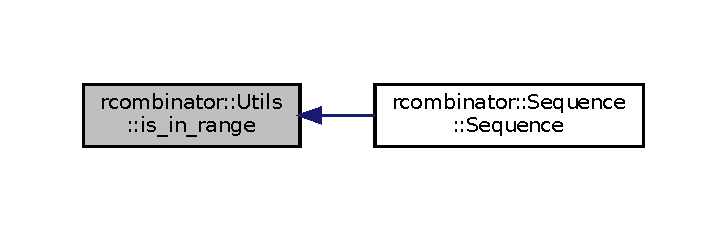
\includegraphics[width=349pt]{namespacercombinator_1_1Utils_aa38fa31292dbf3a06522dc76b20e2572_icgraph}
\end{center}
\end{figure}

\chapter{Class Documentation}
\hypertarget{classrcombinator_1_1Exception}{}\section{rcombinator\+:\+:Exception Class Reference}
\label{classrcombinator_1_1Exception}\index{rcombinator\+::\+Exception@{rcombinator\+::\+Exception}}


Basic class to represent exceptions.  




{\ttfamily \#include $<$exception.\+h$>$}

\subsection*{Public Member Functions}
\begin{DoxyCompactItemize}
\item 
\mbox{\hyperlink{classrcombinator_1_1Exception_a7d3c8825d7c2d7d1d8c9c537725734de}{Exception}} (std\+::string \mbox{\hyperlink{classrcombinator_1_1Exception_a982a342c7c75134b7323ecd67e43e13d}{error\+\_\+msg}})
\begin{DoxyCompactList}\small\item\em Basic constructor for an exception that is to be thrown. \end{DoxyCompactList}\item 
\mbox{\Hypertarget{classrcombinator_1_1Exception_ae91e04f748b6e093c7370ed2b1649d07}\label{classrcombinator_1_1Exception_ae91e04f748b6e093c7370ed2b1649d07}} 
std\+::string \mbox{\hyperlink{classrcombinator_1_1Exception_ae91e04f748b6e093c7370ed2b1649d07}{what}} () const
\begin{DoxyCompactList}\small\item\em The error message for this exception. \end{DoxyCompactList}\end{DoxyCompactItemize}
\subsection*{Private Attributes}
\begin{DoxyCompactItemize}
\item 
\mbox{\Hypertarget{classrcombinator_1_1Exception_a982a342c7c75134b7323ecd67e43e13d}\label{classrcombinator_1_1Exception_a982a342c7c75134b7323ecd67e43e13d}} 
const std\+::string \mbox{\hyperlink{classrcombinator_1_1Exception_a982a342c7c75134b7323ecd67e43e13d}{error\+\_\+msg}}
\begin{DoxyCompactList}\small\item\em A helpful diagnostic message. \end{DoxyCompactList}\end{DoxyCompactItemize}


\subsection{Detailed Description}
Basic class to represent exceptions. 

Stores an error message. 

\subsection{Constructor \& Destructor Documentation}
\mbox{\Hypertarget{classrcombinator_1_1Exception_a7d3c8825d7c2d7d1d8c9c537725734de}\label{classrcombinator_1_1Exception_a7d3c8825d7c2d7d1d8c9c537725734de}} 
\index{rcombinator\+::\+Exception@{rcombinator\+::\+Exception}!Exception@{Exception}}
\index{Exception@{Exception}!rcombinator\+::\+Exception@{rcombinator\+::\+Exception}}
\subsubsection{\texorpdfstring{Exception()}{Exception()}}
{\footnotesize\ttfamily rcombinator\+::\+Exception\+::\+Exception (\begin{DoxyParamCaption}\item[{std\+::string}]{error\+\_\+msg }\end{DoxyParamCaption})\hspace{0.3cm}{\ttfamily [inline]}}



Basic constructor for an exception that is to be thrown. 

Takes the error message as input argument. 

The documentation for this class was generated from the following file\+:\begin{DoxyCompactItemize}
\item 
src/\mbox{\hyperlink{exception_8h}{exception.\+h}}\end{DoxyCompactItemize}

\hypertarget{classrcombinator_1_1F81Model}{}\section{rcombinator\+:\+:F81\+Model Class Reference}
\label{classrcombinator_1_1F81Model}\index{rcombinator\+::\+F81\+Model@{rcombinator\+::\+F81\+Model}}


Felsenstein 1981 Model.  




{\ttfamily \#include $<$point\+\_\+mutation\+\_\+models.\+h$>$}



Inheritance diagram for rcombinator\+:\+:F81\+Model\+:\nopagebreak
\begin{figure}[H]
\begin{center}
\leavevmode
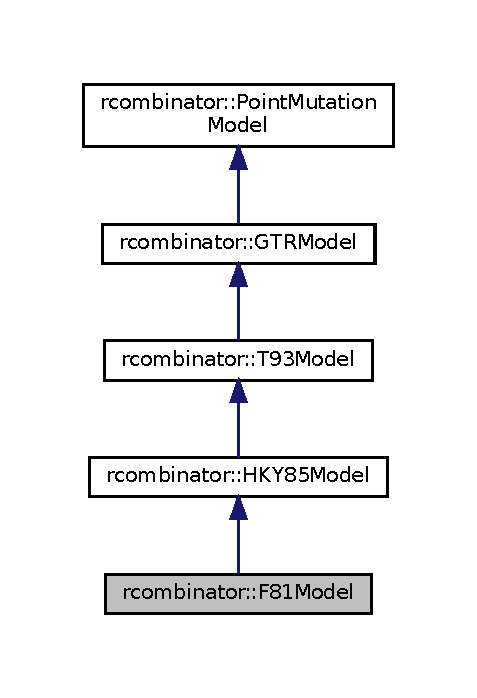
\includegraphics[width=229pt]{classrcombinator_1_1F81Model__inherit__graph}
\end{center}
\end{figure}


Collaboration diagram for rcombinator\+:\+:F81\+Model\+:\nopagebreak
\begin{figure}[H]
\begin{center}
\leavevmode
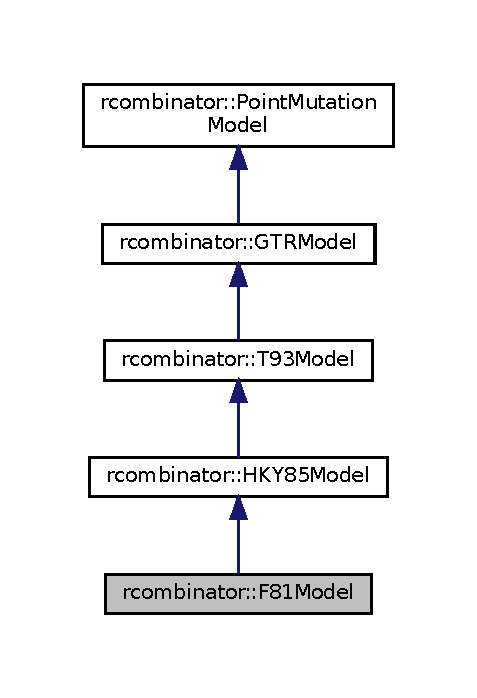
\includegraphics[width=229pt]{classrcombinator_1_1F81Model__coll__graph}
\end{center}
\end{figure}
\subsection*{Public Member Functions}
\begin{DoxyCompactItemize}
\item 
\mbox{\hyperlink{classrcombinator_1_1F81Model_a80c3357497cdc6b91ff4c408750b47bb}{F81\+Model}} (double \mbox{\hyperlink{classrcombinator_1_1GTRModel_a1f58fe556a5ce9aaba6168c9f91e8372}{pi\+\_\+T}}=0.\+25, double pi\+\_\+C=0.\+25, double pi\+\_\+A=0.\+25, double pi\+\_\+G=0.\+25, double \mbox{\hyperlink{classrcombinator_1_1PointMutationModel_a328a30a438bb1b6a625faa3f714a85c8}{scale}}=1)
\begin{DoxyCompactList}\small\item\em 4 equilibrium base frequency parameters and 1 scale parameter. \end{DoxyCompactList}\end{DoxyCompactItemize}
\subsection*{Protected Member Functions}
\begin{DoxyCompactItemize}
\item 
\mbox{\Hypertarget{classrcombinator_1_1F81Model_a5bb9c63e55c4f8f7b9573281ff6ee610}\label{classrcombinator_1_1F81Model_a5bb9c63e55c4f8f7b9573281ff6ee610}} 
void \mbox{\hyperlink{classrcombinator_1_1F81Model_a5bb9c63e55c4f8f7b9573281ff6ee610}{compute\+\_\+transition\+\_\+matrix}} () override
\begin{DoxyCompactList}\small\item\em Computed by exploiting symmetry. \end{DoxyCompactList}\end{DoxyCompactItemize}
\subsection*{Additional Inherited Members}


\subsection{Detailed Description}
Felsenstein 1981 Model. 

\subsection{Constructor \& Destructor Documentation}
\mbox{\Hypertarget{classrcombinator_1_1F81Model_a80c3357497cdc6b91ff4c408750b47bb}\label{classrcombinator_1_1F81Model_a80c3357497cdc6b91ff4c408750b47bb}} 
\index{rcombinator\+::\+F81\+Model@{rcombinator\+::\+F81\+Model}!F81\+Model@{F81\+Model}}
\index{F81\+Model@{F81\+Model}!rcombinator\+::\+F81\+Model@{rcombinator\+::\+F81\+Model}}
\subsubsection{\texorpdfstring{F81\+Model()}{F81Model()}}
{\footnotesize\ttfamily F81\+Model\+::\+F81\+Model (\begin{DoxyParamCaption}\item[{double}]{pi\+\_\+T = {\ttfamily 0.25},  }\item[{double}]{pi\+\_\+C = {\ttfamily 0.25},  }\item[{double}]{pi\+\_\+A = {\ttfamily 0.25},  }\item[{double}]{pi\+\_\+G = {\ttfamily 0.25},  }\item[{double}]{scale = {\ttfamily 1} }\end{DoxyParamCaption})}



4 equilibrium base frequency parameters and 1 scale parameter. 

pi\+\_\+X = same as for G\+TR scale = same as for G\+TR 

The documentation for this class was generated from the following files\+:\begin{DoxyCompactItemize}
\item 
src/\mbox{\hyperlink{point__mutation__models_8h}{point\+\_\+mutation\+\_\+models.\+h}}\item 
src/point\+\_\+mutation\+\_\+models.\+cpp\end{DoxyCompactItemize}

\hypertarget{classrcombinator_1_1GTRModel}{}\section{rcombinator\+:\+:G\+T\+R\+Model Class Reference}
\label{classrcombinator_1_1GTRModel}\index{rcombinator\+::\+G\+T\+R\+Model@{rcombinator\+::\+G\+T\+R\+Model}}


General Time Reversible Model, Tavare 1986.  




{\ttfamily \#include $<$point\+\_\+mutation\+\_\+models.\+h$>$}



Inheritance diagram for rcombinator\+:\+:G\+T\+R\+Model\+:\nopagebreak
\begin{figure}[H]
\begin{center}
\leavevmode
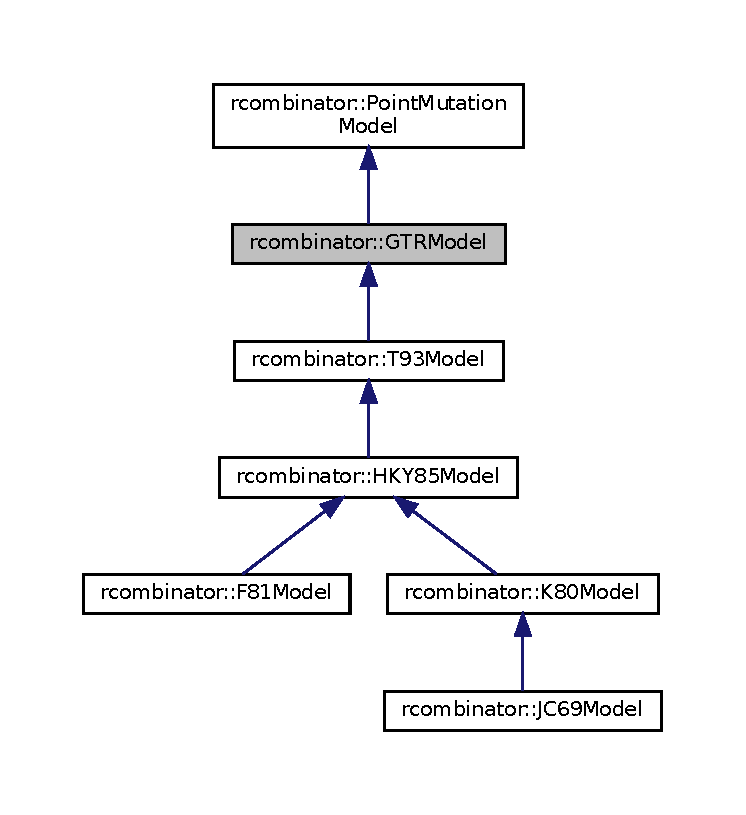
\includegraphics[width=350pt]{classrcombinator_1_1GTRModel__inherit__graph}
\end{center}
\end{figure}


Collaboration diagram for rcombinator\+:\+:G\+T\+R\+Model\+:\nopagebreak
\begin{figure}[H]
\begin{center}
\leavevmode
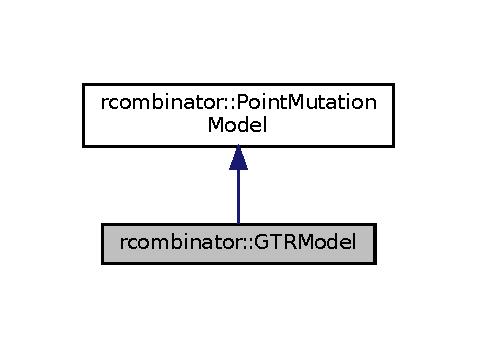
\includegraphics[width=229pt]{classrcombinator_1_1GTRModel__coll__graph}
\end{center}
\end{figure}
\subsection*{Public Member Functions}
\begin{DoxyCompactItemize}
\item 
\mbox{\hyperlink{classrcombinator_1_1GTRModel_addd67a44caae9a477fc986d287dc2e8e}{G\+T\+R\+Model}} (double \mbox{\hyperlink{classrcombinator_1_1GTRModel_a1f58fe556a5ce9aaba6168c9f91e8372}{pi\+\_\+T}}=0.\+25, double pi\+\_\+C=0.\+25, double pi\+\_\+A=0.\+25, double pi\+\_\+G=0.\+25, double T2C=1, double T2A=1, double T2G=1, double C2A=1, double C2G=1, double A2G=1, double \mbox{\hyperlink{classrcombinator_1_1PointMutationModel_a328a30a438bb1b6a625faa3f714a85c8}{scale}}=1)
\begin{DoxyCompactList}\small\item\em 4 equilibrium base frequency parameters, 6 substitution rate parameters and 1 scale parameter. \end{DoxyCompactList}\end{DoxyCompactItemize}
\subsection*{Protected Member Functions}
\begin{DoxyCompactItemize}
\item 
\mbox{\Hypertarget{classrcombinator_1_1GTRModel_a7d71f990fd33bcb7fc6a74accf03d7ae}\label{classrcombinator_1_1GTRModel_a7d71f990fd33bcb7fc6a74accf03d7ae}} 
void \mbox{\hyperlink{classrcombinator_1_1GTRModel_a7d71f990fd33bcb7fc6a74accf03d7ae}{compute\+\_\+transition\+\_\+matrix}} () override
\begin{DoxyCompactList}\small\item\em To be computed using exponentiation of Q. \end{DoxyCompactList}\end{DoxyCompactItemize}
\subsection*{Protected Attributes}
\textbf{ }\par
\begin{DoxyCompactItemize}
\item 
const double \mbox{\hyperlink{classrcombinator_1_1GTRModel_a1f58fe556a5ce9aaba6168c9f91e8372}{pi\+\_\+T}}
\begin{DoxyCompactList}\small\item\em The base frequency parameters. \end{DoxyCompactList}\item 
\mbox{\Hypertarget{classrcombinator_1_1GTRModel_ac601c64807a386c360ecfa78ba2dba18}\label{classrcombinator_1_1GTRModel_ac601c64807a386c360ecfa78ba2dba18}} 
const double {\bfseries pi\+\_\+C}
\item 
\mbox{\Hypertarget{classrcombinator_1_1GTRModel_a8cb703f73d2ee28f85ceaa3459bba8a6}\label{classrcombinator_1_1GTRModel_a8cb703f73d2ee28f85ceaa3459bba8a6}} 
const double {\bfseries pi\+\_\+A}
\item 
\mbox{\Hypertarget{classrcombinator_1_1GTRModel_a249c03ce37700cf0f7374a06e96b2f9e}\label{classrcombinator_1_1GTRModel_a249c03ce37700cf0f7374a06e96b2f9e}} 
const double {\bfseries pi\+\_\+G}
\end{DoxyCompactItemize}

\subsection*{Additional Inherited Members}


\subsection{Detailed Description}
General Time Reversible Model, Tavare 1986. 

\subsection{Constructor \& Destructor Documentation}
\mbox{\Hypertarget{classrcombinator_1_1GTRModel_addd67a44caae9a477fc986d287dc2e8e}\label{classrcombinator_1_1GTRModel_addd67a44caae9a477fc986d287dc2e8e}} 
\index{rcombinator\+::\+G\+T\+R\+Model@{rcombinator\+::\+G\+T\+R\+Model}!G\+T\+R\+Model@{G\+T\+R\+Model}}
\index{G\+T\+R\+Model@{G\+T\+R\+Model}!rcombinator\+::\+G\+T\+R\+Model@{rcombinator\+::\+G\+T\+R\+Model}}
\subsubsection{\texorpdfstring{G\+T\+R\+Model()}{GTRModel()}}
{\footnotesize\ttfamily G\+T\+R\+Model\+::\+G\+T\+R\+Model (\begin{DoxyParamCaption}\item[{double}]{pi\+\_\+T = {\ttfamily 0.25},  }\item[{double}]{pi\+\_\+C = {\ttfamily 0.25},  }\item[{double}]{pi\+\_\+A = {\ttfamily 0.25},  }\item[{double}]{pi\+\_\+G = {\ttfamily 0.25},  }\item[{double}]{T2C = {\ttfamily 1},  }\item[{double}]{T2A = {\ttfamily 1},  }\item[{double}]{T2G = {\ttfamily 1},  }\item[{double}]{C2A = {\ttfamily 1},  }\item[{double}]{C2G = {\ttfamily 1},  }\item[{double}]{A2G = {\ttfamily 1},  }\item[{double}]{scale = {\ttfamily 1} }\end{DoxyParamCaption})}



4 equilibrium base frequency parameters, 6 substitution rate parameters and 1 scale parameter. 

pi\+\_\+X = equilibrium base frequencies X2Y = rate of X becoming Y scale = the scalar by which the matrix is to be scaled to get mutations/million years 

\subsection{Member Data Documentation}
\mbox{\Hypertarget{classrcombinator_1_1GTRModel_a1f58fe556a5ce9aaba6168c9f91e8372}\label{classrcombinator_1_1GTRModel_a1f58fe556a5ce9aaba6168c9f91e8372}} 
\index{rcombinator\+::\+G\+T\+R\+Model@{rcombinator\+::\+G\+T\+R\+Model}!pi\+\_\+T@{pi\+\_\+T}}
\index{pi\+\_\+T@{pi\+\_\+T}!rcombinator\+::\+G\+T\+R\+Model@{rcombinator\+::\+G\+T\+R\+Model}}
\subsubsection{\texorpdfstring{pi\+\_\+T}{pi\_T}}
{\footnotesize\ttfamily const double rcombinator\+::\+G\+T\+R\+Model\+::pi\+\_\+T\hspace{0.3cm}{\ttfamily [protected]}}



The base frequency parameters. 

pi\+\_\+X is the proportion of the sequence that has nucleotide X after the system has reached equilibrium. 

The documentation for this class was generated from the following files\+:\begin{DoxyCompactItemize}
\item 
src/\mbox{\hyperlink{point__mutation__models_8h}{point\+\_\+mutation\+\_\+models.\+h}}\item 
src/point\+\_\+mutation\+\_\+models.\+cpp\end{DoxyCompactItemize}

\hypertarget{classrcombinator_1_1HKY85Model}{}\section{rcombinator\+:\+:H\+K\+Y85\+Model Class Reference}
\label{classrcombinator_1_1HKY85Model}\index{rcombinator\+::\+H\+K\+Y85\+Model@{rcombinator\+::\+H\+K\+Y85\+Model}}


Hasegawa, Kishino and Yano 1985 Model.  




{\ttfamily \#include $<$point\+\_\+mutation\+\_\+models.\+h$>$}



Inheritance diagram for rcombinator\+:\+:H\+K\+Y85\+Model\+:\nopagebreak
\begin{figure}[H]
\begin{center}
\leavevmode
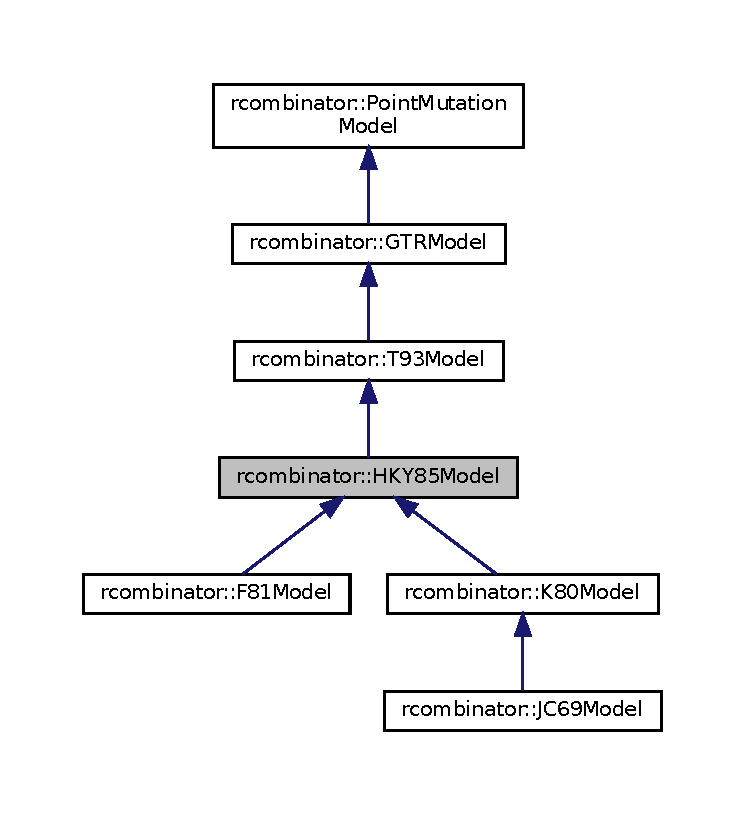
\includegraphics[width=350pt]{classrcombinator_1_1HKY85Model__inherit__graph}
\end{center}
\end{figure}


Collaboration diagram for rcombinator\+:\+:H\+K\+Y85\+Model\+:\nopagebreak
\begin{figure}[H]
\begin{center}
\leavevmode
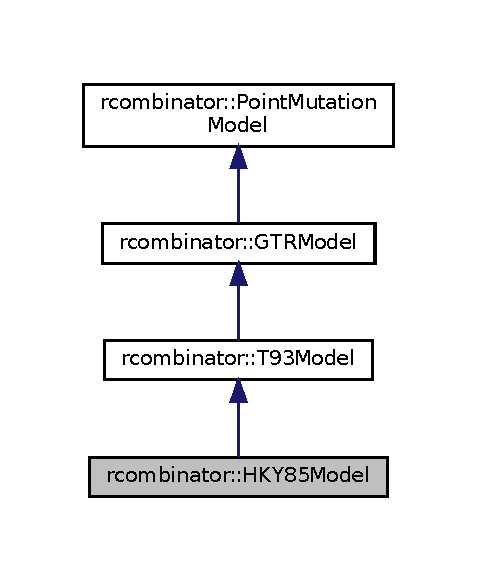
\includegraphics[width=229pt]{classrcombinator_1_1HKY85Model__coll__graph}
\end{center}
\end{figure}
\subsection*{Public Member Functions}
\begin{DoxyCompactItemize}
\item 
\mbox{\hyperlink{classrcombinator_1_1HKY85Model_aba3aea50215010285dd40b4093bf55c1}{H\+K\+Y85\+Model}} (double pi\+\_\+T=0.\+25, double pi\+\_\+C=0.\+25, double pi\+\_\+A=0.\+25, double pi\+\_\+G=0.\+25, double k=0.\+1, double \mbox{\hyperlink{classrcombinator_1_1PointMutationModel_a328a30a438bb1b6a625faa3f714a85c8}{scale}}=0.\+25)
\item 
\mbox{\Hypertarget{classrcombinator_1_1HKY85Model_a156ac5c3789bc479857299469269c4de}\label{classrcombinator_1_1HKY85Model_a156ac5c3789bc479857299469269c4de}} 
double $\ast$$\ast$ \mbox{\hyperlink{classrcombinator_1_1HKY85Model_a156ac5c3789bc479857299469269c4de}{get\+\_\+transition\+\_\+matrix}} (double t) override
\begin{DoxyCompactList}\small\item\em To be computed using exponentiation of Q. \end{DoxyCompactList}\end{DoxyCompactItemize}
\subsection*{Additional Inherited Members}


\subsection{Detailed Description}
Hasegawa, Kishino and Yano 1985 Model. 

\subsection{Constructor \& Destructor Documentation}
\mbox{\Hypertarget{classrcombinator_1_1HKY85Model_aba3aea50215010285dd40b4093bf55c1}\label{classrcombinator_1_1HKY85Model_aba3aea50215010285dd40b4093bf55c1}} 
\index{rcombinator\+::\+H\+K\+Y85\+Model@{rcombinator\+::\+H\+K\+Y85\+Model}!H\+K\+Y85\+Model@{H\+K\+Y85\+Model}}
\index{H\+K\+Y85\+Model@{H\+K\+Y85\+Model}!rcombinator\+::\+H\+K\+Y85\+Model@{rcombinator\+::\+H\+K\+Y85\+Model}}
\subsubsection{\texorpdfstring{H\+K\+Y85\+Model()}{HKY85Model()}}
{\footnotesize\ttfamily H\+K\+Y85\+Model\+::\+H\+K\+Y85\+Model (\begin{DoxyParamCaption}\item[{double}]{pi\+\_\+T = {\ttfamily 0.25},  }\item[{double}]{pi\+\_\+C = {\ttfamily 0.25},  }\item[{double}]{pi\+\_\+A = {\ttfamily 0.25},  }\item[{double}]{pi\+\_\+G = {\ttfamily 0.25},  }\item[{double}]{k = {\ttfamily 0.1},  }\item[{double}]{scale = {\ttfamily 0.25} }\end{DoxyParamCaption})}

\begin{DoxyRefDesc}{Todo}
\item[\mbox{\hyperlink{todo__todo000004}{Todo}}]Use the defaults from \mbox{\hyperlink{constants_8h}{constants.\+h}} \end{DoxyRefDesc}


The documentation for this class was generated from the following files\+:\begin{DoxyCompactItemize}
\item 
src/\mbox{\hyperlink{point__mutation__models_8h}{point\+\_\+mutation\+\_\+models.\+h}}\item 
src/point\+\_\+mutation\+\_\+models.\+cpp\end{DoxyCompactItemize}

\hypertarget{classrcombinator_1_1JC69Model}{}\section{rcombinator\+:\+:J\+C69\+Model Class Reference}
\label{classrcombinator_1_1JC69Model}\index{rcombinator\+::\+J\+C69\+Model@{rcombinator\+::\+J\+C69\+Model}}


Jules and Cantor, 1969.  




{\ttfamily \#include $<$point\+\_\+mutation\+\_\+models.\+h$>$}



Inheritance diagram for rcombinator\+:\+:J\+C69\+Model\+:\nopagebreak
\begin{figure}[H]
\begin{center}
\leavevmode
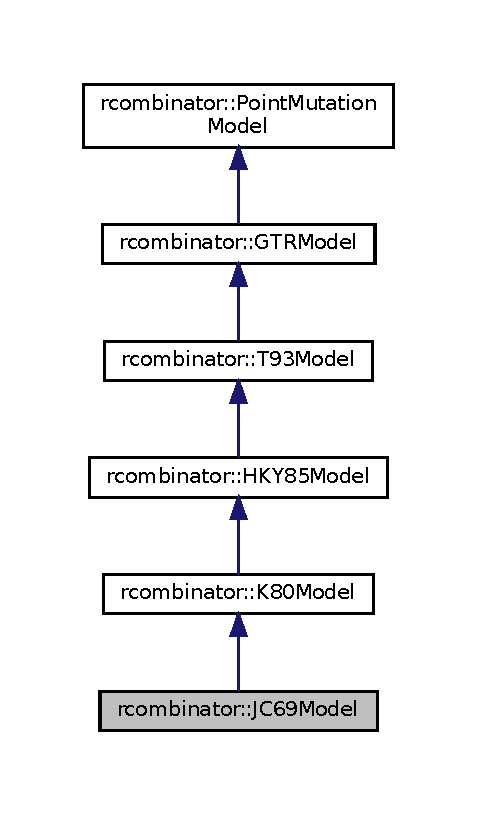
\includegraphics[width=229pt]{classrcombinator_1_1JC69Model__inherit__graph}
\end{center}
\end{figure}


Collaboration diagram for rcombinator\+:\+:J\+C69\+Model\+:\nopagebreak
\begin{figure}[H]
\begin{center}
\leavevmode
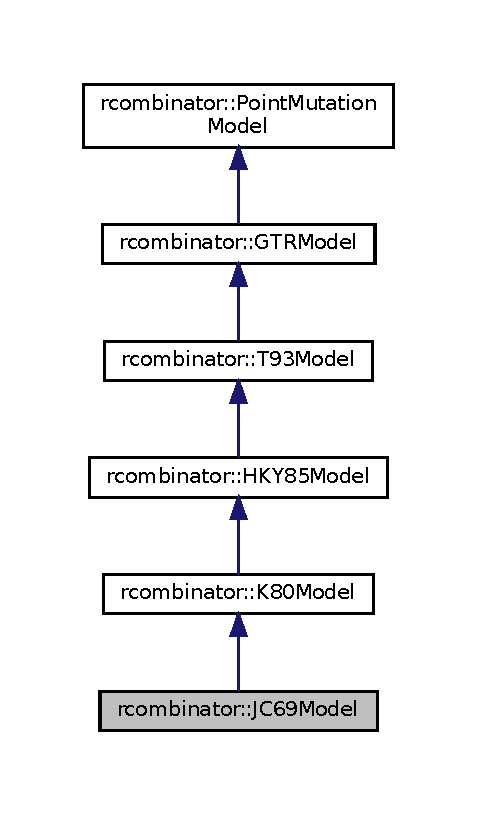
\includegraphics[width=229pt]{classrcombinator_1_1JC69Model__coll__graph}
\end{center}
\end{figure}
\subsection*{Public Member Functions}
\begin{DoxyCompactItemize}
\item 
\mbox{\hyperlink{classrcombinator_1_1JC69Model_a979834f85de8b2bb92d0cce5e64d6346}{J\+C69\+Model}} (double \mbox{\hyperlink{classrcombinator_1_1PointMutationModel_a328a30a438bb1b6a625faa3f714a85c8}{scale}}=0.\+25)
\end{DoxyCompactItemize}
\subsection*{Additional Inherited Members}


\subsection{Detailed Description}
Jules and Cantor, 1969. 

\subsection{Constructor \& Destructor Documentation}
\mbox{\Hypertarget{classrcombinator_1_1JC69Model_a979834f85de8b2bb92d0cce5e64d6346}\label{classrcombinator_1_1JC69Model_a979834f85de8b2bb92d0cce5e64d6346}} 
\index{rcombinator\+::\+J\+C69\+Model@{rcombinator\+::\+J\+C69\+Model}!J\+C69\+Model@{J\+C69\+Model}}
\index{J\+C69\+Model@{J\+C69\+Model}!rcombinator\+::\+J\+C69\+Model@{rcombinator\+::\+J\+C69\+Model}}
\subsubsection{\texorpdfstring{J\+C69\+Model()}{JC69Model()}}
{\footnotesize\ttfamily J\+C69\+Model\+::\+J\+C69\+Model (\begin{DoxyParamCaption}\item[{double}]{scale = {\ttfamily 0.25} }\end{DoxyParamCaption})}

\begin{DoxyRefDesc}{Todo}
\item[\mbox{\hyperlink{todo__todo000007}{Todo}}]Use the defaults from \mbox{\hyperlink{constants_8h}{constants.\+h}} \end{DoxyRefDesc}


The documentation for this class was generated from the following files\+:\begin{DoxyCompactItemize}
\item 
src/\mbox{\hyperlink{point__mutation__models_8h}{point\+\_\+mutation\+\_\+models.\+h}}\item 
src/point\+\_\+mutation\+\_\+models.\+cpp\end{DoxyCompactItemize}

\hypertarget{classrcombinator_1_1K80Model}{}\section{rcombinator\+:\+:K80\+Model Class Reference}
\label{classrcombinator_1_1K80Model}\index{rcombinator\+::\+K80\+Model@{rcombinator\+::\+K80\+Model}}


Kimura 2 Parameter Model, 1980.  




{\ttfamily \#include $<$point\+\_\+mutation\+\_\+models.\+h$>$}



Inheritance diagram for rcombinator\+:\+:K80\+Model\+:\nopagebreak
\begin{figure}[H]
\begin{center}
\leavevmode
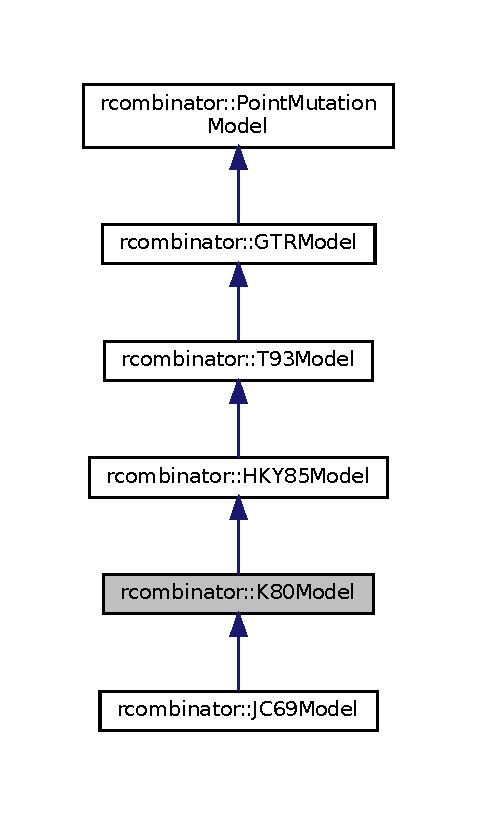
\includegraphics[width=229pt]{classrcombinator_1_1K80Model__inherit__graph}
\end{center}
\end{figure}


Collaboration diagram for rcombinator\+:\+:K80\+Model\+:\nopagebreak
\begin{figure}[H]
\begin{center}
\leavevmode
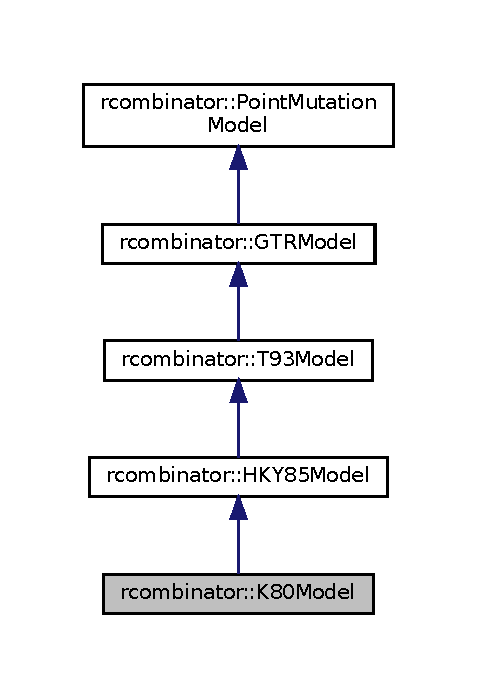
\includegraphics[width=229pt]{classrcombinator_1_1K80Model__coll__graph}
\end{center}
\end{figure}
\subsection*{Public Member Functions}
\begin{DoxyCompactItemize}
\item 
\mbox{\hyperlink{classrcombinator_1_1K80Model_af199581e9a4d387f5e9e4f5bd048904b}{K80\+Model}} (double k=\mbox{\hyperlink{namespacercombinator_1_1Consts_af2e735f6e0661176144a8769131b8aa7}{Consts\+::\+K80\+\_\+K}}, double \mbox{\hyperlink{classrcombinator_1_1PointMutationModel_a328a30a438bb1b6a625faa3f714a85c8}{scale}}=Consts\+::\+K80\+\_\+\+S\+C\+A\+LE)
\begin{DoxyCompactList}\small\item\em 1 substitution rate parameter and 1 scale parameter. \end{DoxyCompactList}\end{DoxyCompactItemize}
\subsection*{Protected Member Functions}
\begin{DoxyCompactItemize}
\item 
\mbox{\Hypertarget{classrcombinator_1_1K80Model_a70f669e2a31d34a37b19fd185219a9ce}\label{classrcombinator_1_1K80Model_a70f669e2a31d34a37b19fd185219a9ce}} 
void \mbox{\hyperlink{classrcombinator_1_1K80Model_a70f669e2a31d34a37b19fd185219a9ce}{compute\+\_\+transition\+\_\+matrix}} () override
\begin{DoxyCompactList}\small\item\em Computed by exploiting symmetry. \end{DoxyCompactList}\end{DoxyCompactItemize}
\subsection*{Additional Inherited Members}


\subsection{Detailed Description}
Kimura 2 Parameter Model, 1980. 

\subsection{Constructor \& Destructor Documentation}
\mbox{\Hypertarget{classrcombinator_1_1K80Model_af199581e9a4d387f5e9e4f5bd048904b}\label{classrcombinator_1_1K80Model_af199581e9a4d387f5e9e4f5bd048904b}} 
\index{rcombinator\+::\+K80\+Model@{rcombinator\+::\+K80\+Model}!K80\+Model@{K80\+Model}}
\index{K80\+Model@{K80\+Model}!rcombinator\+::\+K80\+Model@{rcombinator\+::\+K80\+Model}}
\subsubsection{\texorpdfstring{K80\+Model()}{K80Model()}}
{\footnotesize\ttfamily K80\+Model\+::\+K80\+Model (\begin{DoxyParamCaption}\item[{double}]{k = {\ttfamily \mbox{\hyperlink{namespacercombinator_1_1Consts_af2e735f6e0661176144a8769131b8aa7}{Consts\+::\+K80\+\_\+K}}},  }\item[{double}]{scale = {\ttfamily Consts\+:\+:K80\+\_\+SCALE} }\end{DoxyParamCaption})}



1 substitution rate parameter and 1 scale parameter. 

k = rate of transitions (assuming rate of transversions is 1) scale = same as for G\+TR 

The documentation for this class was generated from the following files\+:\begin{DoxyCompactItemize}
\item 
src/\mbox{\hyperlink{point__mutation__models_8h}{point\+\_\+mutation\+\_\+models.\+h}}\item 
src/point\+\_\+mutation\+\_\+models.\+cpp\end{DoxyCompactItemize}

\hypertarget{classrcombinator_1_1PointMutationModel}{}\section{rcombinator\+:\+:Point\+Mutation\+Model Class Reference}
\label{classrcombinator_1_1PointMutationModel}\index{rcombinator\+::\+Point\+Mutation\+Model@{rcombinator\+::\+Point\+Mutation\+Model}}


To represent a model of D\+NA evolution through point mutations.  




{\ttfamily \#include $<$point\+\_\+mutation\+\_\+models.\+h$>$}



Inheritance diagram for rcombinator\+:\+:Point\+Mutation\+Model\+:\nopagebreak
\begin{figure}[H]
\begin{center}
\leavevmode
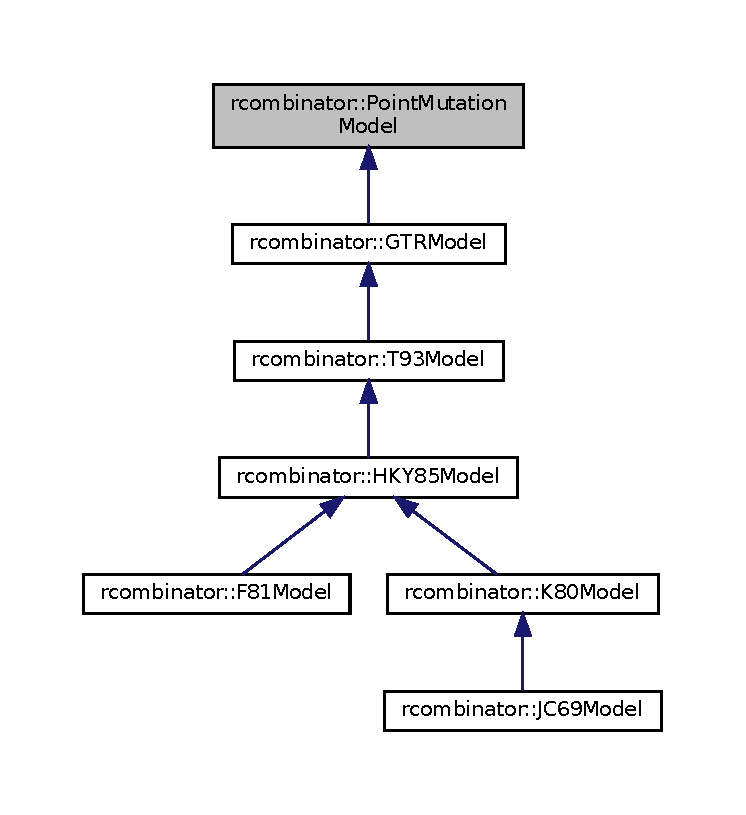
\includegraphics[width=350pt]{classrcombinator_1_1PointMutationModel__inherit__graph}
\end{center}
\end{figure}
\subsection*{Public Member Functions}
\begin{DoxyCompactItemize}
\item 
\mbox{\Hypertarget{classrcombinator_1_1PointMutationModel_a099dd1d991389c50d1e22f6d25dc913d}\label{classrcombinator_1_1PointMutationModel_a099dd1d991389c50d1e22f6d25dc913d}} 
\mbox{\hyperlink{classrcombinator_1_1PointMutationModel_a099dd1d991389c50d1e22f6d25dc913d}{Point\+Mutation\+Model}} (double \mbox{\hyperlink{classrcombinator_1_1PointMutationModel_a328a30a438bb1b6a625faa3f714a85c8}{scale}}=0.\+25)
\begin{DoxyCompactList}\small\item\em Constructor that allocates memory for transition matrix. \end{DoxyCompactList}\item 
virtual \mbox{\hyperlink{classrcombinator_1_1PointMutationModel_a2ac7ebc4b6264c6597808574501e45e5}{$\sim$\+Point\+Mutation\+Model}} ()
\begin{DoxyCompactList}\small\item\em Destructor that allocates memory for transition matrix. \end{DoxyCompactList}\item 
double $\ast$$\ast$ \mbox{\hyperlink{classrcombinator_1_1PointMutationModel_a43457739c51566273d471098dc2cacf0}{get\+\_\+Q}} ()
\begin{DoxyCompactList}\small\item\em Returns a rate matrix for the mutations. \end{DoxyCompactList}\item 
virtual double $\ast$$\ast$ \mbox{\hyperlink{classrcombinator_1_1PointMutationModel_a35a8b397c8fa932cd870174aa45180da}{get\+\_\+transition\+\_\+matrix}} (double t)=0
\begin{DoxyCompactList}\small\item\em Returns a transition matrix to represent the probabilities of mutations from each nucleotide to the other. \end{DoxyCompactList}\end{DoxyCompactItemize}
\subsection*{Protected Attributes}
\begin{DoxyCompactItemize}
\item 
\mbox{\Hypertarget{classrcombinator_1_1PointMutationModel_a5affb482b1e4434bd1b2c6fc1c579934}\label{classrcombinator_1_1PointMutationModel_a5affb482b1e4434bd1b2c6fc1c579934}} 
double $\ast$$\ast$ \mbox{\hyperlink{classrcombinator_1_1PointMutationModel_a5affb482b1e4434bd1b2c6fc1c579934}{Q\+\_\+mat}}
\begin{DoxyCompactList}\small\item\em The transition rate matrix. \end{DoxyCompactList}\item 
\mbox{\Hypertarget{classrcombinator_1_1PointMutationModel_a328a30a438bb1b6a625faa3f714a85c8}\label{classrcombinator_1_1PointMutationModel_a328a30a438bb1b6a625faa3f714a85c8}} 
double \mbox{\hyperlink{classrcombinator_1_1PointMutationModel_a328a30a438bb1b6a625faa3f714a85c8}{scale}}
\begin{DoxyCompactList}\small\item\em How much to scale Q by in the differential equation. \end{DoxyCompactList}\item 
\mbox{\Hypertarget{classrcombinator_1_1PointMutationModel_a8ae23bc482a483e139cdb94bdc332a72}\label{classrcombinator_1_1PointMutationModel_a8ae23bc482a483e139cdb94bdc332a72}} 
double \mbox{\hyperlink{classrcombinator_1_1PointMutationModel_a8ae23bc482a483e139cdb94bdc332a72}{t\+\_\+stored}}
\begin{DoxyCompactList}\small\item\em The timestep by which we jump in our simulation. \end{DoxyCompactList}\item 
\mbox{\Hypertarget{classrcombinator_1_1PointMutationModel_ac8ec41d0bffdc2221ad4b1cfb06424e8}\label{classrcombinator_1_1PointMutationModel_ac8ec41d0bffdc2221ad4b1cfb06424e8}} 
double $\ast$$\ast$ \mbox{\hyperlink{classrcombinator_1_1PointMutationModel_ac8ec41d0bffdc2221ad4b1cfb06424e8}{T\+\_\+mat}}
\begin{DoxyCompactList}\small\item\em The transition matrix for timestep {\itshape t}. \end{DoxyCompactList}\end{DoxyCompactItemize}


\subsection{Detailed Description}
To represent a model of D\+NA evolution through point mutations. 

\subsection{Constructor \& Destructor Documentation}
\mbox{\Hypertarget{classrcombinator_1_1PointMutationModel_a2ac7ebc4b6264c6597808574501e45e5}\label{classrcombinator_1_1PointMutationModel_a2ac7ebc4b6264c6597808574501e45e5}} 
\index{rcombinator\+::\+Point\+Mutation\+Model@{rcombinator\+::\+Point\+Mutation\+Model}!````~Point\+Mutation\+Model@{$\sim$\+Point\+Mutation\+Model}}
\index{````~Point\+Mutation\+Model@{$\sim$\+Point\+Mutation\+Model}!rcombinator\+::\+Point\+Mutation\+Model@{rcombinator\+::\+Point\+Mutation\+Model}}
\subsubsection{\texorpdfstring{$\sim$\+Point\+Mutation\+Model()}{~PointMutationModel()}}
{\footnotesize\ttfamily Point\+Mutation\+Model\+::$\sim$\+Point\+Mutation\+Model (\begin{DoxyParamCaption}{ }\end{DoxyParamCaption})\hspace{0.3cm}{\ttfamily [virtual]}}



Destructor that allocates memory for transition matrix. 

Is virtual because we want all specific point mutation models to derive from this class. 

\subsection{Member Function Documentation}
\mbox{\Hypertarget{classrcombinator_1_1PointMutationModel_a43457739c51566273d471098dc2cacf0}\label{classrcombinator_1_1PointMutationModel_a43457739c51566273d471098dc2cacf0}} 
\index{rcombinator\+::\+Point\+Mutation\+Model@{rcombinator\+::\+Point\+Mutation\+Model}!get\+\_\+Q@{get\+\_\+Q}}
\index{get\+\_\+Q@{get\+\_\+Q}!rcombinator\+::\+Point\+Mutation\+Model@{rcombinator\+::\+Point\+Mutation\+Model}}
\subsubsection{\texorpdfstring{get\+\_\+\+Q()}{get\_Q()}}
{\footnotesize\ttfamily double$\ast$$\ast$ rcombinator\+::\+Point\+Mutation\+Model\+::get\+\_\+Q (\begin{DoxyParamCaption}{ }\end{DoxyParamCaption})\hspace{0.3cm}{\ttfamily [inline]}}



Returns a rate matrix for the mutations. 

After {\itshape t} years have passed, the probability is exp(rate$\ast$t). \mbox{\Hypertarget{classrcombinator_1_1PointMutationModel_a35a8b397c8fa932cd870174aa45180da}\label{classrcombinator_1_1PointMutationModel_a35a8b397c8fa932cd870174aa45180da}} 
\index{rcombinator\+::\+Point\+Mutation\+Model@{rcombinator\+::\+Point\+Mutation\+Model}!get\+\_\+transition\+\_\+matrix@{get\+\_\+transition\+\_\+matrix}}
\index{get\+\_\+transition\+\_\+matrix@{get\+\_\+transition\+\_\+matrix}!rcombinator\+::\+Point\+Mutation\+Model@{rcombinator\+::\+Point\+Mutation\+Model}}
\subsubsection{\texorpdfstring{get\+\_\+transition\+\_\+matrix()}{get\_transition\_matrix()}}
{\footnotesize\ttfamily virtual double$\ast$$\ast$ rcombinator\+::\+Point\+Mutation\+Model\+::get\+\_\+transition\+\_\+matrix (\begin{DoxyParamCaption}\item[{double}]{t }\end{DoxyParamCaption})\hspace{0.3cm}{\ttfamily [pure virtual]}}



Returns a transition matrix to represent the probabilities of mutations from each nucleotide to the other. 

{\itshape t} is the time that has passed. P(\+A to B) is matrix(\+A, B). 

Implemented in \mbox{\hyperlink{classrcombinator_1_1K80Model_a35aec33b0b090ab23dc7e0985d1bedf5}{rcombinator\+::\+K80\+Model}}, \mbox{\hyperlink{classrcombinator_1_1F81Model_a7b8cc2e77bd7d15582aaa77aa876755c}{rcombinator\+::\+F81\+Model}}, \mbox{\hyperlink{classrcombinator_1_1HKY85Model_a156ac5c3789bc479857299469269c4de}{rcombinator\+::\+H\+K\+Y85\+Model}}, \mbox{\hyperlink{classrcombinator_1_1T93Model_ac8e280547d6af408e24df5e114d2c5c9}{rcombinator\+::\+T93\+Model}}, and \mbox{\hyperlink{classrcombinator_1_1GTRModel_aca26ae97d8ee3af6cc3c372d4d606e64}{rcombinator\+::\+G\+T\+R\+Model}}.

Here is the caller graph for this function\+:\nopagebreak
\begin{figure}[H]
\begin{center}
\leavevmode
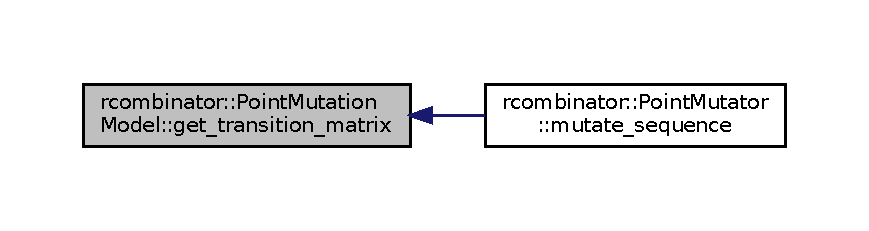
\includegraphics[width=350pt]{classrcombinator_1_1PointMutationModel_a35a8b397c8fa932cd870174aa45180da_icgraph}
\end{center}
\end{figure}


The documentation for this class was generated from the following files\+:\begin{DoxyCompactItemize}
\item 
src/\mbox{\hyperlink{point__mutation__models_8h}{point\+\_\+mutation\+\_\+models.\+h}}\item 
src/point\+\_\+mutation\+\_\+models.\+cpp\end{DoxyCompactItemize}

\hypertarget{classrcombinator_1_1PointMutator}{}\section{rcombinator\+:\+:Point\+Mutator Class Reference}
\label{classrcombinator_1_1PointMutator}\index{rcombinator\+::\+Point\+Mutator@{rcombinator\+::\+Point\+Mutator}}


A class that can mutate a given sequence according to a specified point mutation model.  




{\ttfamily \#include $<$point\+\_\+mutator.\+h$>$}



Collaboration diagram for rcombinator\+:\+:Point\+Mutator\+:\nopagebreak
\begin{figure}[H]
\begin{center}
\leavevmode
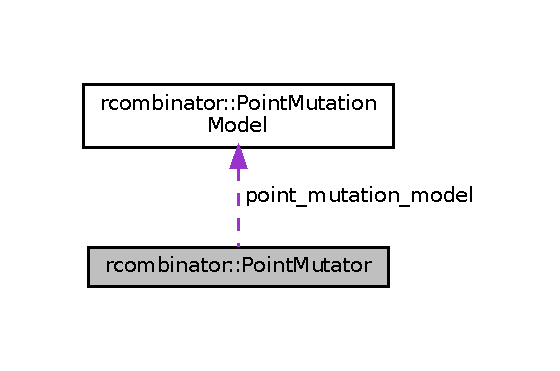
\includegraphics[width=269pt]{classrcombinator_1_1PointMutator__coll__graph}
\end{center}
\end{figure}
\subsection*{Public Member Functions}
\begin{DoxyCompactItemize}
\item 
\mbox{\Hypertarget{classrcombinator_1_1PointMutator_a084f37ad47f0a820028a87695bd2c88e}\label{classrcombinator_1_1PointMutator_a084f37ad47f0a820028a87695bd2c88e}} 
\mbox{\hyperlink{classrcombinator_1_1PointMutator_a084f37ad47f0a820028a87695bd2c88e}{Point\+Mutator}} (std\+::string model, \mbox{\hyperlink{constants_8h_abcd18a5521fc90ff6e7b00e4fee98397}{size\+\_\+type}} n, \mbox{\hyperlink{constants_8h_abcd18a5521fc90ff6e7b00e4fee98397}{size\+\_\+type}} num\+\_\+sensitive\+\_\+posns=0, double inactive\+\_\+probability=0.\+0)
\begin{DoxyCompactList}\small\item\em Constructor that chooses a point mutation model and the probabilities for lethal mutations at each position in the sequence. \end{DoxyCompactList}\item 
\mbox{\Hypertarget{classrcombinator_1_1PointMutator_ab4bb79937f1824e7fba92fb824f27c56}\label{classrcombinator_1_1PointMutator_ab4bb79937f1824e7fba92fb824f27c56}} 
\mbox{\hyperlink{classrcombinator_1_1PointMutator_ab4bb79937f1824e7fba92fb824f27c56}{$\sim$\+Point\+Mutator}} ()
\begin{DoxyCompactList}\small\item\em Destructor that frees up memory. \end{DoxyCompactList}\item 
\mbox{\Hypertarget{classrcombinator_1_1PointMutator_aba3c2b8641affe8a06d815c33cafdc1b}\label{classrcombinator_1_1PointMutator_aba3c2b8641affe8a06d815c33cafdc1b}} 
void \mbox{\hyperlink{classrcombinator_1_1PointMutator_aba3c2b8641affe8a06d815c33cafdc1b}{mutate\+\_\+sequence}} (\mbox{\hyperlink{classrcombinator_1_1Sequence}{Sequence}} \&s, double timestep) const
\begin{DoxyCompactList}\small\item\em Mutates a sequence according to a given transition matrix. \end{DoxyCompactList}\end{DoxyCompactItemize}
\subsection*{Private Attributes}
\begin{DoxyCompactItemize}
\item 
\mbox{\Hypertarget{classrcombinator_1_1PointMutator_a2e6661ed12c29646de00485b10bd8c74}\label{classrcombinator_1_1PointMutator_a2e6661ed12c29646de00485b10bd8c74}} 
\mbox{\hyperlink{classrcombinator_1_1PointMutationModel}{Point\+Mutation\+Model}} $\ast$ \mbox{\hyperlink{classrcombinator_1_1PointMutator_a2e6661ed12c29646de00485b10bd8c74}{point\+\_\+mutation\+\_\+model}}
\begin{DoxyCompactList}\small\item\em Which point mutation model this mutator coressponds to. \end{DoxyCompactList}\item 
\mbox{\Hypertarget{classrcombinator_1_1PointMutator_a0c3e0e7165db72541b331246603d545b}\label{classrcombinator_1_1PointMutator_a0c3e0e7165db72541b331246603d545b}} 
std\+::vector$<$ double $>$ \mbox{\hyperlink{classrcombinator_1_1PointMutator_a0c3e0e7165db72541b331246603d545b}{lethal\+\_\+mutation\+\_\+probs}}
\begin{DoxyCompactList}\small\item\em What is the probability that a mutation at a given position results in inactivity. \end{DoxyCompactList}\end{DoxyCompactItemize}


\subsection{Detailed Description}
A class that can mutate a given sequence according to a specified point mutation model. 

We need to specify how long the sequence has evolved for. 

The documentation for this class was generated from the following files\+:\begin{DoxyCompactItemize}
\item 
src/\mbox{\hyperlink{point__mutator_8h}{point\+\_\+mutator.\+h}}\item 
src/point\+\_\+mutator.\+cpp\end{DoxyCompactItemize}

\hypertarget{classrcombinator_1_1RandMaths}{}\section{rcombinator\+:\+:Rand\+Maths Class Reference}
\label{classrcombinator_1_1RandMaths}\index{rcombinator\+::\+Rand\+Maths@{rcombinator\+::\+Rand\+Maths}}


For all maths helper functions that use random number generation.  




{\ttfamily \#include $<$rand\+\_\+maths.\+h$>$}

\subsection*{Public Member Functions}
\begin{DoxyCompactItemize}
\item 
int \mbox{\hyperlink{classrcombinator_1_1RandMaths_ae417da209eb8a9d1b2217e7a5397926c}{rand\+\_\+int}} (int low, int high)
\begin{DoxyCompactList}\small\item\em Generates a random integer within a range. \end{DoxyCompactList}\item 
double \mbox{\hyperlink{classrcombinator_1_1RandMaths_aa6441baa59bff50f588c0c54e3c54140}{rand\+\_\+real}} (double low=0.\+0, double high=1.\+0)
\begin{DoxyCompactList}\small\item\em Generates a random real number within a range. \end{DoxyCompactList}\item 
long \mbox{\hyperlink{classrcombinator_1_1RandMaths_a1fec117f0ebd5a7834fdcf649a23edd7}{rand\+\_\+poisson}} (double mean)
\begin{DoxyCompactList}\small\item\em Chooses a number sampled from a Poisson distribution. \end{DoxyCompactList}\item 
std\+::set$<$ int $>$ \mbox{\hyperlink{classrcombinator_1_1RandMaths_a2c31949c9ac03952cb0006e6a88e3d85}{sample\+\_\+without\+\_\+replacement}} (int low, int high, int m)
\begin{DoxyCompactList}\small\item\em Samples {\itshape m} integers within a range, without replacement. \end{DoxyCompactList}\item 
std\+::pair$<$ int, int $>$ \mbox{\hyperlink{classrcombinator_1_1RandMaths_aaa759efa3059b6793100cb6b6442f26d}{sample\+\_\+distinct\+\_\+pair}} (int low, int high)
\begin{DoxyCompactList}\small\item\em Samples a non-\/diagonal pair (2 distinct values) within a range. \end{DoxyCompactList}\item 
bool \mbox{\hyperlink{classrcombinator_1_1RandMaths_a183686140a9da18ad40c7e048ee8914e}{test\+\_\+event}} (double event\+\_\+probability)
\begin{DoxyCompactList}\small\item\em Tests whether or not an event happened. \end{DoxyCompactList}\item 
int \mbox{\hyperlink{classrcombinator_1_1RandMaths_afbc0d35bd9744ecab1983914ac32d68c}{choose\+\_\+event}} (double $\ast$events, long num\+\_\+events)
\begin{DoxyCompactList}\small\item\em Chooses an event from a list of possible events. \end{DoxyCompactList}\end{DoxyCompactItemize}
\textbf{ }\par
\begin{DoxyCompactItemize}
\item 
\mbox{\hyperlink{classrcombinator_1_1RandMaths_ac9b350a4aa07b739dcc2bb12c3b5c0e5}{Rand\+Maths}} (\mbox{\hyperlink{classrcombinator_1_1RandMaths}{Rand\+Maths}} const \&)=delete
\begin{DoxyCompactList}\small\item\em Delete copy constructors as want \mbox{\hyperlink{classrcombinator_1_1RandMaths}{Rand\+Maths}} to be a singleton. \end{DoxyCompactList}\item 
\mbox{\Hypertarget{classrcombinator_1_1RandMaths_ab26d84d79d640cd343ac3e94a70ad184}\label{classrcombinator_1_1RandMaths_ab26d84d79d640cd343ac3e94a70ad184}} 
void {\bfseries operator=} (\mbox{\hyperlink{classrcombinator_1_1RandMaths}{Rand\+Maths}} const \&)=delete
\end{DoxyCompactItemize}

\subsection*{Static Public Member Functions}
\begin{DoxyCompactItemize}
\item 
static \mbox{\hyperlink{classrcombinator_1_1RandMaths}{Rand\+Maths}} \& \mbox{\hyperlink{classrcombinator_1_1RandMaths_aa96396651fba75ffb972b5fa1c2994c7}{initialize\+Rand\+Maths}} (long seed=0)
\begin{DoxyCompactList}\small\item\em Returns an instance of a \mbox{\hyperlink{classrcombinator_1_1RandMaths}{Rand\+Maths}} class, after seeding it. \end{DoxyCompactList}\end{DoxyCompactItemize}


\subsection{Detailed Description}
For all maths helper functions that use random number generation. 

This is implemented as a singleton that can either be specifically seeded (for testing and debugging) or can be randomly seeded (for simulations). 

\subsection{Constructor \& Destructor Documentation}
\mbox{\Hypertarget{classrcombinator_1_1RandMaths_ac9b350a4aa07b739dcc2bb12c3b5c0e5}\label{classrcombinator_1_1RandMaths_ac9b350a4aa07b739dcc2bb12c3b5c0e5}} 
\index{rcombinator\+::\+Rand\+Maths@{rcombinator\+::\+Rand\+Maths}!Rand\+Maths@{Rand\+Maths}}
\index{Rand\+Maths@{Rand\+Maths}!rcombinator\+::\+Rand\+Maths@{rcombinator\+::\+Rand\+Maths}}
\subsubsection{\texorpdfstring{Rand\+Maths()}{RandMaths()}}
{\footnotesize\ttfamily rcombinator\+::\+Rand\+Maths\+::\+Rand\+Maths (\begin{DoxyParamCaption}\item[{\mbox{\hyperlink{classrcombinator_1_1RandMaths}{Rand\+Maths}} const \&}]{ }\end{DoxyParamCaption})\hspace{0.3cm}{\ttfamily [delete]}}



Delete copy constructors as want \mbox{\hyperlink{classrcombinator_1_1RandMaths}{Rand\+Maths}} to be a singleton. 

The reason these are public is because most compilers check for private-\/ness before they check to see if functions are deleted, and we want our error messages to be helpful if we create a new \mbox{\hyperlink{classrcombinator_1_1RandMaths}{Rand\+Maths}} object by mistake. 

\subsection{Member Function Documentation}
\mbox{\Hypertarget{classrcombinator_1_1RandMaths_afbc0d35bd9744ecab1983914ac32d68c}\label{classrcombinator_1_1RandMaths_afbc0d35bd9744ecab1983914ac32d68c}} 
\index{rcombinator\+::\+Rand\+Maths@{rcombinator\+::\+Rand\+Maths}!choose\+\_\+event@{choose\+\_\+event}}
\index{choose\+\_\+event@{choose\+\_\+event}!rcombinator\+::\+Rand\+Maths@{rcombinator\+::\+Rand\+Maths}}
\subsubsection{\texorpdfstring{choose\+\_\+event()}{choose\_event()}}
{\footnotesize\ttfamily int Rand\+Maths\+::choose\+\_\+event (\begin{DoxyParamCaption}\item[{double $\ast$}]{events,  }\item[{long}]{num\+\_\+events }\end{DoxyParamCaption})}



Chooses an event from a list of possible events. 

Takes the probabilities of each of the events as input. Throws an exception if the probabilites do not add up to at least 1.

\begin{DoxyRefDesc}{Todo}
\item[\mbox{\hyperlink{todo__todo000001}{Todo}}]Make this a safe pointer rather than a raw one, or use a vector rather than a raw array.\end{DoxyRefDesc}


\begin{DoxyRefDesc}{Todo}
\item[\mbox{\hyperlink{todo__todo000002}{Todo}}]Throw an exception even if probabilities add up to something greater than 1. \end{DoxyRefDesc}
Here is the call graph for this function\+:
\nopagebreak
\begin{figure}[H]
\begin{center}
\leavevmode
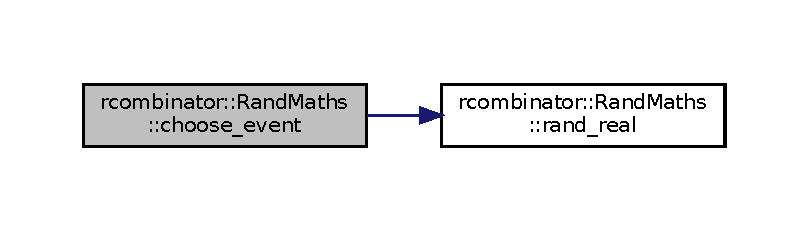
\includegraphics[width=350pt]{classrcombinator_1_1RandMaths_afbc0d35bd9744ecab1983914ac32d68c_cgraph}
\end{center}
\end{figure}
\mbox{\Hypertarget{classrcombinator_1_1RandMaths_aa96396651fba75ffb972b5fa1c2994c7}\label{classrcombinator_1_1RandMaths_aa96396651fba75ffb972b5fa1c2994c7}} 
\index{rcombinator\+::\+Rand\+Maths@{rcombinator\+::\+Rand\+Maths}!initialize\+Rand\+Maths@{initialize\+Rand\+Maths}}
\index{initialize\+Rand\+Maths@{initialize\+Rand\+Maths}!rcombinator\+::\+Rand\+Maths@{rcombinator\+::\+Rand\+Maths}}
\subsubsection{\texorpdfstring{initialize\+Rand\+Maths()}{initializeRandMaths()}}
{\footnotesize\ttfamily \mbox{\hyperlink{classrcombinator_1_1RandMaths}{Rand\+Maths}} \& Rand\+Maths\+::initialize\+Rand\+Maths (\begin{DoxyParamCaption}\item[{long}]{seed = {\ttfamily 0} }\end{DoxyParamCaption})\hspace{0.3cm}{\ttfamily [static]}}



Returns an instance of a \mbox{\hyperlink{classrcombinator_1_1RandMaths}{Rand\+Maths}} class, after seeding it. 

Can be done only once as we want to share the random number generation among all other classes, and seed only once for controlling the numbers that are generated. If the seed is set to the special value 0 during construction, the seed is randomly chosen using system time. \mbox{\Hypertarget{classrcombinator_1_1RandMaths_ae417da209eb8a9d1b2217e7a5397926c}\label{classrcombinator_1_1RandMaths_ae417da209eb8a9d1b2217e7a5397926c}} 
\index{rcombinator\+::\+Rand\+Maths@{rcombinator\+::\+Rand\+Maths}!rand\+\_\+int@{rand\+\_\+int}}
\index{rand\+\_\+int@{rand\+\_\+int}!rcombinator\+::\+Rand\+Maths@{rcombinator\+::\+Rand\+Maths}}
\subsubsection{\texorpdfstring{rand\+\_\+int()}{rand\_int()}}
{\footnotesize\ttfamily int Rand\+Maths\+::rand\+\_\+int (\begin{DoxyParamCaption}\item[{int}]{low,  }\item[{int}]{high }\end{DoxyParamCaption})}



Generates a random integer within a range. 

The bounds are \mbox{[}inclusive\+\_\+low, exclusive\+\_\+high). Here is the caller graph for this function\+:
\nopagebreak
\begin{figure}[H]
\begin{center}
\leavevmode
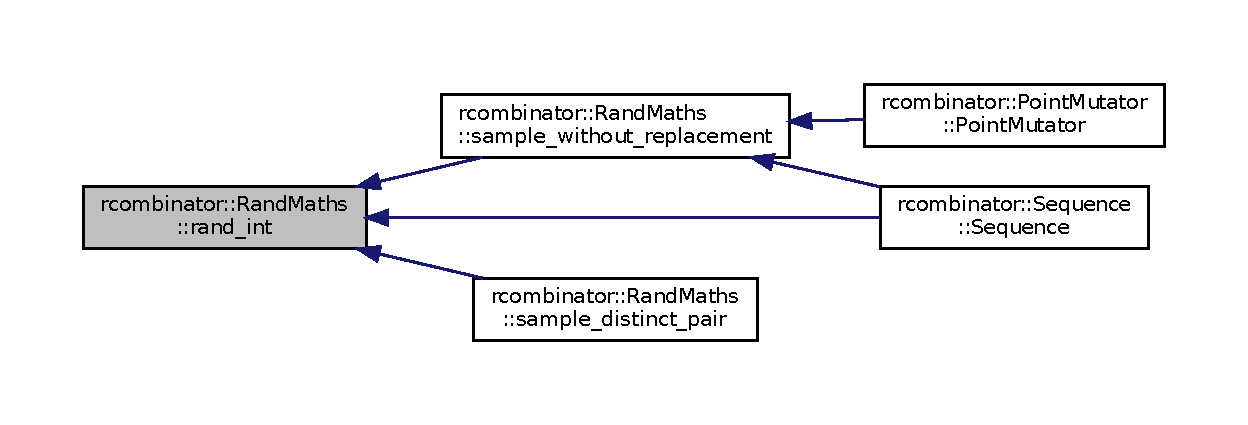
\includegraphics[width=350pt]{classrcombinator_1_1RandMaths_ae417da209eb8a9d1b2217e7a5397926c_icgraph}
\end{center}
\end{figure}
\mbox{\Hypertarget{classrcombinator_1_1RandMaths_a1fec117f0ebd5a7834fdcf649a23edd7}\label{classrcombinator_1_1RandMaths_a1fec117f0ebd5a7834fdcf649a23edd7}} 
\index{rcombinator\+::\+Rand\+Maths@{rcombinator\+::\+Rand\+Maths}!rand\+\_\+poisson@{rand\+\_\+poisson}}
\index{rand\+\_\+poisson@{rand\+\_\+poisson}!rcombinator\+::\+Rand\+Maths@{rcombinator\+::\+Rand\+Maths}}
\subsubsection{\texorpdfstring{rand\+\_\+poisson()}{rand\_poisson()}}
{\footnotesize\ttfamily long Rand\+Maths\+::rand\+\_\+poisson (\begin{DoxyParamCaption}\item[{double}]{mean }\end{DoxyParamCaption})}



Chooses a number sampled from a Poisson distribution. 

Takes the mean as a parameter. \mbox{\Hypertarget{classrcombinator_1_1RandMaths_aa6441baa59bff50f588c0c54e3c54140}\label{classrcombinator_1_1RandMaths_aa6441baa59bff50f588c0c54e3c54140}} 
\index{rcombinator\+::\+Rand\+Maths@{rcombinator\+::\+Rand\+Maths}!rand\+\_\+real@{rand\+\_\+real}}
\index{rand\+\_\+real@{rand\+\_\+real}!rcombinator\+::\+Rand\+Maths@{rcombinator\+::\+Rand\+Maths}}
\subsubsection{\texorpdfstring{rand\+\_\+real()}{rand\_real()}}
{\footnotesize\ttfamily double Rand\+Maths\+::rand\+\_\+real (\begin{DoxyParamCaption}\item[{double}]{low = {\ttfamily 0.0},  }\item[{double}]{high = {\ttfamily 1.0} }\end{DoxyParamCaption})}



Generates a random real number within a range. 

The bounds are \mbox{[}inclusive\+\_\+low, exclusive high). Here is the caller graph for this function\+:
\nopagebreak
\begin{figure}[H]
\begin{center}
\leavevmode
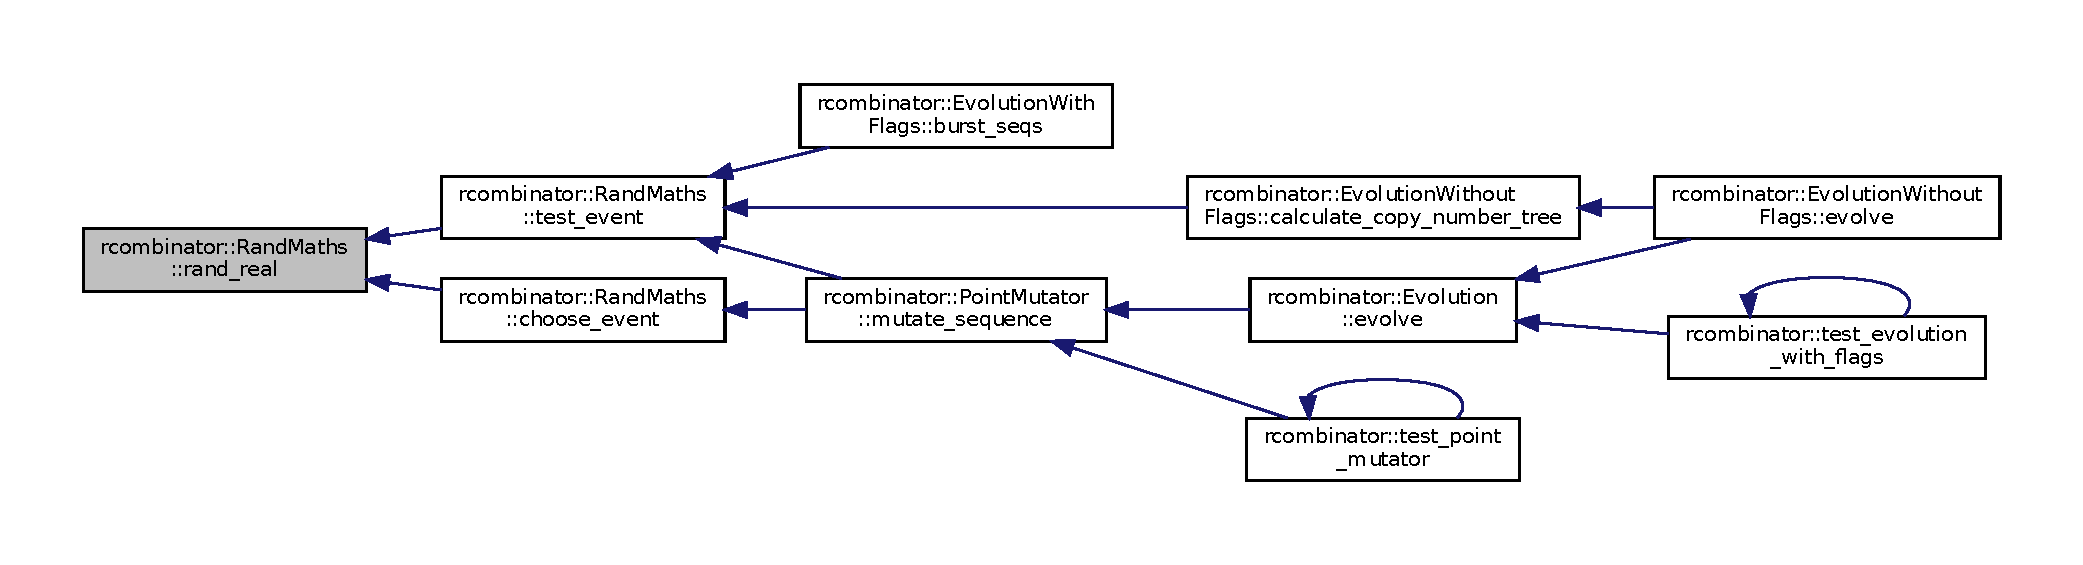
\includegraphics[width=350pt]{classrcombinator_1_1RandMaths_aa6441baa59bff50f588c0c54e3c54140_icgraph}
\end{center}
\end{figure}
\mbox{\Hypertarget{classrcombinator_1_1RandMaths_aaa759efa3059b6793100cb6b6442f26d}\label{classrcombinator_1_1RandMaths_aaa759efa3059b6793100cb6b6442f26d}} 
\index{rcombinator\+::\+Rand\+Maths@{rcombinator\+::\+Rand\+Maths}!sample\+\_\+distinct\+\_\+pair@{sample\+\_\+distinct\+\_\+pair}}
\index{sample\+\_\+distinct\+\_\+pair@{sample\+\_\+distinct\+\_\+pair}!rcombinator\+::\+Rand\+Maths@{rcombinator\+::\+Rand\+Maths}}
\subsubsection{\texorpdfstring{sample\+\_\+distinct\+\_\+pair()}{sample\_distinct\_pair()}}
{\footnotesize\ttfamily std\+::pair$<$ int, int $>$ Rand\+Maths\+::sample\+\_\+distinct\+\_\+pair (\begin{DoxyParamCaption}\item[{int}]{low,  }\item[{int}]{high }\end{DoxyParamCaption})}



Samples a non-\/diagonal pair (2 distinct values) within a range. 

The bounds for each value are \mbox{[}inclusive\+\_\+low, exclusive high). Here is the call graph for this function\+:
\nopagebreak
\begin{figure}[H]
\begin{center}
\leavevmode
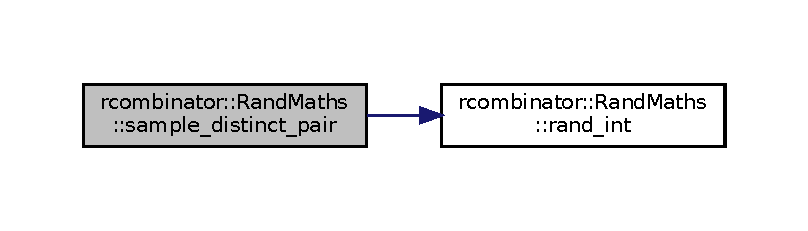
\includegraphics[width=350pt]{classrcombinator_1_1RandMaths_aaa759efa3059b6793100cb6b6442f26d_cgraph}
\end{center}
\end{figure}
\mbox{\Hypertarget{classrcombinator_1_1RandMaths_a2c31949c9ac03952cb0006e6a88e3d85}\label{classrcombinator_1_1RandMaths_a2c31949c9ac03952cb0006e6a88e3d85}} 
\index{rcombinator\+::\+Rand\+Maths@{rcombinator\+::\+Rand\+Maths}!sample\+\_\+without\+\_\+replacement@{sample\+\_\+without\+\_\+replacement}}
\index{sample\+\_\+without\+\_\+replacement@{sample\+\_\+without\+\_\+replacement}!rcombinator\+::\+Rand\+Maths@{rcombinator\+::\+Rand\+Maths}}
\subsubsection{\texorpdfstring{sample\+\_\+without\+\_\+replacement()}{sample\_without\_replacement()}}
{\footnotesize\ttfamily std\+::set$<$ int $>$ Rand\+Maths\+::sample\+\_\+without\+\_\+replacement (\begin{DoxyParamCaption}\item[{int}]{low,  }\item[{int}]{high,  }\item[{int}]{m }\end{DoxyParamCaption})}



Samples {\itshape m} integers within a range, without replacement. 

The bounds are \mbox{[}inclusive\+\_\+low, exclusive high). The integers are returned in ascending order. Here is the call graph for this function\+:
\nopagebreak
\begin{figure}[H]
\begin{center}
\leavevmode
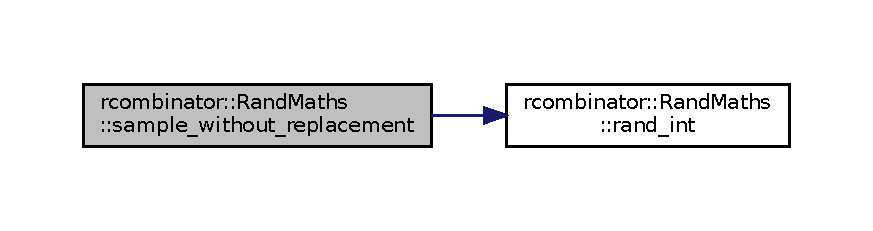
\includegraphics[width=350pt]{classrcombinator_1_1RandMaths_a2c31949c9ac03952cb0006e6a88e3d85_cgraph}
\end{center}
\end{figure}
\mbox{\Hypertarget{classrcombinator_1_1RandMaths_a183686140a9da18ad40c7e048ee8914e}\label{classrcombinator_1_1RandMaths_a183686140a9da18ad40c7e048ee8914e}} 
\index{rcombinator\+::\+Rand\+Maths@{rcombinator\+::\+Rand\+Maths}!test\+\_\+event@{test\+\_\+event}}
\index{test\+\_\+event@{test\+\_\+event}!rcombinator\+::\+Rand\+Maths@{rcombinator\+::\+Rand\+Maths}}
\subsubsection{\texorpdfstring{test\+\_\+event()}{test\_event()}}
{\footnotesize\ttfamily bool Rand\+Maths\+::test\+\_\+event (\begin{DoxyParamCaption}\item[{double}]{event\+\_\+probability }\end{DoxyParamCaption})\hspace{0.3cm}{\ttfamily [inline]}}



Tests whether or not an event happened. 

Takes the probability of an event as paramter, and then compares it to a random value in \mbox{[}0, 1). Here is the call graph for this function\+:
\nopagebreak
\begin{figure}[H]
\begin{center}
\leavevmode
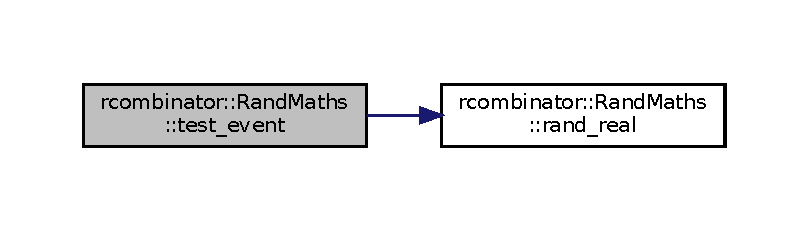
\includegraphics[width=350pt]{classrcombinator_1_1RandMaths_a183686140a9da18ad40c7e048ee8914e_cgraph}
\end{center}
\end{figure}


The documentation for this class was generated from the following files\+:\begin{DoxyCompactItemize}
\item 
src/\mbox{\hyperlink{rand__maths_8h}{rand\+\_\+maths.\+h}}\item 
src/rand\+\_\+maths.\+cpp\end{DoxyCompactItemize}

\hypertarget{classrcombinator_1_1Sequence}{}\section{rcombinator\+:\+:Sequence Class Reference}
\label{classrcombinator_1_1Sequence}\index{rcombinator\+::\+Sequence@{rcombinator\+::\+Sequence}}


To represent a D\+NA sequence and the mutations that it has undergone.  




{\ttfamily \#include $<$sequence.\+h$>$}

\subsection*{Public Member Functions}
\begin{DoxyCompactItemize}
\item 
\mbox{\hyperlink{classrcombinator_1_1Sequence_afab8bafaf1283f4e699ba9111ee452b3}{Sequence}} (long n)
\begin{DoxyCompactList}\small\item\em Constructs a random sequence of length {\itshape n}. \end{DoxyCompactList}\item 
\mbox{\hyperlink{classrcombinator_1_1Sequence_af5b3b62eba07f0e09f532fcf1681c289}{Sequence}} (std\+::string s)
\begin{DoxyCompactList}\small\item\em Constructs a sequence from a given string. \end{DoxyCompactList}\item 
\mbox{\hyperlink{classrcombinator_1_1Sequence_a976b331689ec55d9d306281bbff5d22d}{Sequence}} (\mbox{\hyperlink{classrcombinator_1_1Sequence}{Sequence}} \&s1, \mbox{\hyperlink{classrcombinator_1_1Sequence}{Sequence}} \&s2, int num\+\_\+template\+\_\+switches)
\begin{DoxyCompactList}\small\item\em Constructs a sequence from recombining two other sequences. \end{DoxyCompactList}\item 
\mbox{\Hypertarget{classrcombinator_1_1Sequence_a690c3f7adffafdf45056b5ae632c515d}\label{classrcombinator_1_1Sequence_a690c3f7adffafdf45056b5ae632c515d}} 
long \mbox{\hyperlink{classrcombinator_1_1Sequence_a690c3f7adffafdf45056b5ae632c515d}{get\+\_\+length}} () const
\begin{DoxyCompactList}\small\item\em Returns length of the sequence. \end{DoxyCompactList}\item 
\mbox{\Hypertarget{classrcombinator_1_1Sequence_a5690b6b125807696c81533e7be0be296}\label{classrcombinator_1_1Sequence_a5690b6b125807696c81533e7be0be296}} 
long \mbox{\hyperlink{classrcombinator_1_1Sequence_a5690b6b125807696c81533e7be0be296}{get\+\_\+tag}} () const
\begin{DoxyCompactList}\small\item\em Returns the unique label for this sequence. \end{DoxyCompactList}\item 
\mbox{\Hypertarget{classrcombinator_1_1Sequence_a1367e984a24069fb18f4eb85f5c55dbb}\label{classrcombinator_1_1Sequence_a1367e984a24069fb18f4eb85f5c55dbb}} 
std\+::pair$<$ bool, bool $>$ \mbox{\hyperlink{classrcombinator_1_1Sequence_a1367e984a24069fb18f4eb85f5c55dbb}{bits\+\_\+at}} (long n) const
\begin{DoxyCompactList}\small\item\em Returns the 2bit encoding for a base at a given position. \end{DoxyCompactList}\item 
\mbox{\Hypertarget{classrcombinator_1_1Sequence_a19672a1fbefcdf0c317fddb177f80a15}\label{classrcombinator_1_1Sequence_a19672a1fbefcdf0c317fddb177f80a15}} 
char \mbox{\hyperlink{classrcombinator_1_1Sequence_a19672a1fbefcdf0c317fddb177f80a15}{char\+\_\+at}} (long n) const
\begin{DoxyCompactList}\small\item\em Returns the character for a base at a given position. \end{DoxyCompactList}\item 
void \mbox{\hyperlink{classrcombinator_1_1Sequence_a5f7bccd4725bb8c46f6b93bd01a6b2f0}{point\+\_\+mutate}} (long n, char new\+\_\+nucleotide, bool is\+\_\+lethal=false)
\begin{DoxyCompactList}\small\item\em Changes the nucleotide at position {\itshape n} to {\itshape new\+\_\+nucleotide}. \end{DoxyCompactList}\item 
\mbox{\Hypertarget{classrcombinator_1_1Sequence_a5fa45e155a1e4b3c257f19369ace05a8}\label{classrcombinator_1_1Sequence_a5fa45e155a1e4b3c257f19369ace05a8}} 
std\+::string \mbox{\hyperlink{classrcombinator_1_1Sequence_a5fa45e155a1e4b3c257f19369ace05a8}{as\+\_\+string}} () const
\begin{DoxyCompactList}\small\item\em Returns the raw nucleotide sequence as a string. \end{DoxyCompactList}\item 
bool \mbox{\hyperlink{classrcombinator_1_1Sequence_a5af66ddd3c8bc05307b56737c56060bf}{is\+\_\+active}} () const
\begin{DoxyCompactList}\small\item\em Tests whether this sequence is active (can transpose) or not. \end{DoxyCompactList}\item 
\mbox{\Hypertarget{classrcombinator_1_1Sequence_a821299743e342f028cf7cff51289e3cf}\label{classrcombinator_1_1Sequence_a821299743e342f028cf7cff51289e3cf}} 
long \mbox{\hyperlink{classrcombinator_1_1Sequence_a821299743e342f028cf7cff51289e3cf}{num\+\_\+mutations}} () const
\begin{DoxyCompactList}\small\item\em Returns how many mutations are present in this sequence. \end{DoxyCompactList}\end{DoxyCompactItemize}
\subsection*{Private Types}
\textbf{ }\par
\begin{DoxyCompactItemize}
\item 
typedef std\+::unordered\+\_\+map$<$ long, char $>$ \mbox{\hyperlink{classrcombinator_1_1Sequence_a95c6d1eea79f9551118a4c988433e5b7}{mutations\+\_\+type}}
\begin{DoxyCompactList}\small\item\em Basic typedefs -\/ hashed data structures for quick lookup. \end{DoxyCompactList}\item 
\mbox{\Hypertarget{classrcombinator_1_1Sequence_ae5b0638255a262292d6f4bb31367fc90}\label{classrcombinator_1_1Sequence_ae5b0638255a262292d6f4bb31367fc90}} 
typedef std\+::unordered\+\_\+set$<$ long $>$ {\bfseries lethal\+\_\+mutations\+\_\+type}
\end{DoxyCompactItemize}

\subsection*{Private Attributes}
\begin{DoxyCompactItemize}
\item 
long \mbox{\hyperlink{classrcombinator_1_1Sequence_a9f9a2f4654d8b0e0cdb3061b9e0775d7}{tag}}
\begin{DoxyCompactList}\small\item\em A number that uniquely identifies this sequence. \end{DoxyCompactList}\item 
std\+::vector$<$ bool $>$ \mbox{\hyperlink{classrcombinator_1_1Sequence_ab37aa0bdc97b3d923407e3a7e17b3209}{bases}}
\begin{DoxyCompactList}\small\item\em Actual sequence of nucleotides. \end{DoxyCompactList}\item 
\mbox{\hyperlink{classrcombinator_1_1Sequence_a95c6d1eea79f9551118a4c988433e5b7}{mutations\+\_\+type}} \mbox{\hyperlink{classrcombinator_1_1Sequence_a8aac49ef635b95fe0088e5fb59e2bce7}{mutations}}
\begin{DoxyCompactList}\small\item\em Positions of mutations and what the {\itshape original} nucleotide was. \end{DoxyCompactList}\item 
lethal\+\_\+mutations\+\_\+type \mbox{\hyperlink{classrcombinator_1_1Sequence_abbef2567c1f68239c80769db85455b00}{lethal\+\_\+mutations}}
\begin{DoxyCompactList}\small\item\em Positions of mutations that are lethal. \end{DoxyCompactList}\end{DoxyCompactItemize}
\subsection*{Static Private Attributes}
\begin{DoxyCompactItemize}
\item 
static long \mbox{\hyperlink{classrcombinator_1_1Sequence_abb45023862671bbc450bdea543e72165}{global\+\_\+sequence\+\_\+count}} = 0
\begin{DoxyCompactList}\small\item\em An internal counter that is incremented every time a sequence is created. \end{DoxyCompactList}\end{DoxyCompactItemize}
\subsection*{Friends}
\begin{DoxyCompactItemize}
\item 
long \mbox{\hyperlink{classrcombinator_1_1Sequence_abdc71a8f6617dcb6ab73f0e07eb63b67}{operator$\ast$}} (const \mbox{\hyperlink{classrcombinator_1_1Sequence}{Sequence}} \&s1, const \mbox{\hyperlink{classrcombinator_1_1Sequence}{Sequence}} \&s2)
\begin{DoxyCompactList}\small\item\em Computes pairwise distances between two sequences. \end{DoxyCompactList}\end{DoxyCompactItemize}


\subsection{Detailed Description}
To represent a D\+NA sequence and the mutations that it has undergone. 

Keeps track of the actual sequence, mutations and lethal mutations. 

\subsection{Member Typedef Documentation}
\mbox{\Hypertarget{classrcombinator_1_1Sequence_a95c6d1eea79f9551118a4c988433e5b7}\label{classrcombinator_1_1Sequence_a95c6d1eea79f9551118a4c988433e5b7}} 
\index{rcombinator\+::\+Sequence@{rcombinator\+::\+Sequence}!mutations\+\_\+type@{mutations\+\_\+type}}
\index{mutations\+\_\+type@{mutations\+\_\+type}!rcombinator\+::\+Sequence@{rcombinator\+::\+Sequence}}
\subsubsection{\texorpdfstring{mutations\+\_\+type}{mutations\_type}}
{\footnotesize\ttfamily typedef std\+::unordered\+\_\+map$<$long, char$>$ \mbox{\hyperlink{classrcombinator_1_1Sequence_a95c6d1eea79f9551118a4c988433e5b7}{rcombinator\+::\+Sequence\+::mutations\+\_\+type}}\hspace{0.3cm}{\ttfamily [private]}}



Basic typedefs -\/ hashed data structures for quick lookup. 

For keeping track of mutations and lethal mutations. 

\subsection{Constructor \& Destructor Documentation}
\mbox{\Hypertarget{classrcombinator_1_1Sequence_afab8bafaf1283f4e699ba9111ee452b3}\label{classrcombinator_1_1Sequence_afab8bafaf1283f4e699ba9111ee452b3}} 
\index{rcombinator\+::\+Sequence@{rcombinator\+::\+Sequence}!Sequence@{Sequence}}
\index{Sequence@{Sequence}!rcombinator\+::\+Sequence@{rcombinator\+::\+Sequence}}
\subsubsection{\texorpdfstring{Sequence()}{Sequence()}\hspace{0.1cm}{\footnotesize\ttfamily [1/3]}}
{\footnotesize\ttfamily Sequence\+::\+Sequence (\begin{DoxyParamCaption}\item[{long}]{n }\end{DoxyParamCaption})}



Constructs a random sequence of length {\itshape n}. 

This is considered initial, so no mutations are present. Here is the call graph for this function\+:\nopagebreak
\begin{figure}[H]
\begin{center}
\leavevmode
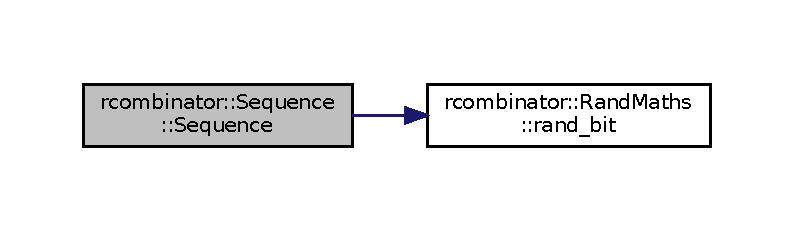
\includegraphics[width=350pt]{classrcombinator_1_1Sequence_afab8bafaf1283f4e699ba9111ee452b3_cgraph}
\end{center}
\end{figure}
\mbox{\Hypertarget{classrcombinator_1_1Sequence_af5b3b62eba07f0e09f532fcf1681c289}\label{classrcombinator_1_1Sequence_af5b3b62eba07f0e09f532fcf1681c289}} 
\index{rcombinator\+::\+Sequence@{rcombinator\+::\+Sequence}!Sequence@{Sequence}}
\index{Sequence@{Sequence}!rcombinator\+::\+Sequence@{rcombinator\+::\+Sequence}}
\subsubsection{\texorpdfstring{Sequence()}{Sequence()}\hspace{0.1cm}{\footnotesize\ttfamily [2/3]}}
{\footnotesize\ttfamily Sequence\+::\+Sequence (\begin{DoxyParamCaption}\item[{std\+::string}]{s }\end{DoxyParamCaption})}



Constructs a sequence from a given string. 

This is considered initial, so no mutations are present. Here is the call graph for this function\+:\nopagebreak
\begin{figure}[H]
\begin{center}
\leavevmode
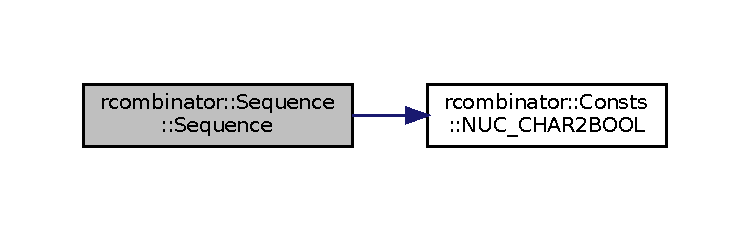
\includegraphics[width=350pt]{classrcombinator_1_1Sequence_af5b3b62eba07f0e09f532fcf1681c289_cgraph}
\end{center}
\end{figure}
\mbox{\Hypertarget{classrcombinator_1_1Sequence_a976b331689ec55d9d306281bbff5d22d}\label{classrcombinator_1_1Sequence_a976b331689ec55d9d306281bbff5d22d}} 
\index{rcombinator\+::\+Sequence@{rcombinator\+::\+Sequence}!Sequence@{Sequence}}
\index{Sequence@{Sequence}!rcombinator\+::\+Sequence@{rcombinator\+::\+Sequence}}
\subsubsection{\texorpdfstring{Sequence()}{Sequence()}\hspace{0.1cm}{\footnotesize\ttfamily [3/3]}}
{\footnotesize\ttfamily Sequence\+::\+Sequence (\begin{DoxyParamCaption}\item[{\mbox{\hyperlink{classrcombinator_1_1Sequence}{Sequence}} \&}]{s1,  }\item[{\mbox{\hyperlink{classrcombinator_1_1Sequence}{Sequence}} \&}]{s2,  }\item[{int}]{num\+\_\+template\+\_\+switches }\end{DoxyParamCaption})}



Constructs a sequence from recombining two other sequences. 

The number of template switches has to be specified, and the positions at which the template switches are made is random.

The mutations recorded are with respect to the original sequences. That is, the new sequence {\itshape s\+\_\+new} will have a mutation {\itshape m} at position {\itshape l} if and only if the sequence {\itshape s\+\_\+old} whose nucleotide is used for {\itshape s\+\_\+new} at position {\itshape l} had mutation {\itshape m} present at that position.

\begin{DoxyRefDesc}{Todo}
\item[\mbox{\hyperlink{todo__todo000010}{Todo}}]Add an option for specifying the positions of the template switches too, or overload this function. \end{DoxyRefDesc}
Here is the call graph for this function\+:\nopagebreak
\begin{figure}[H]
\begin{center}
\leavevmode
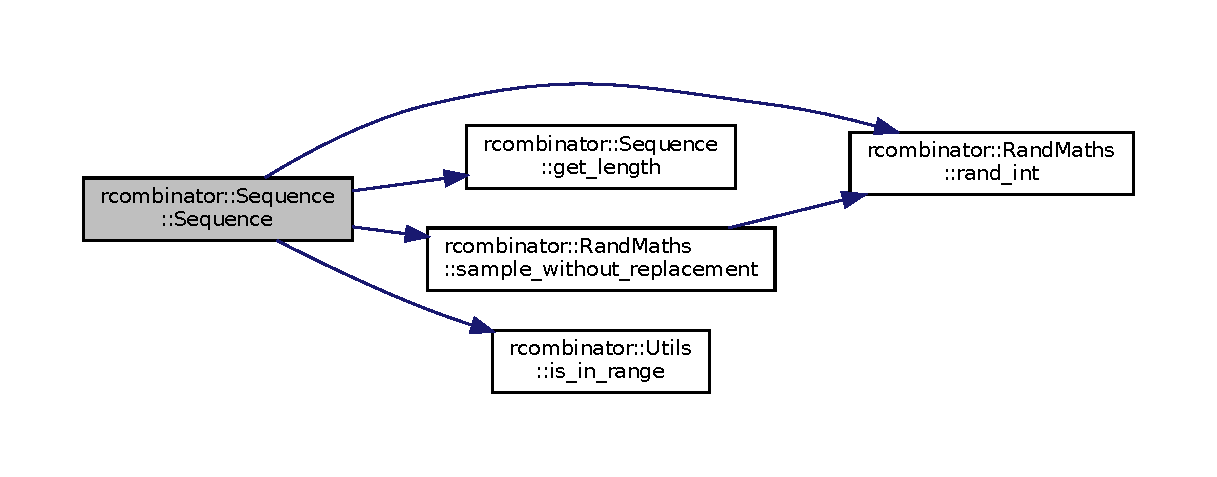
\includegraphics[width=350pt]{classrcombinator_1_1Sequence_a976b331689ec55d9d306281bbff5d22d_cgraph}
\end{center}
\end{figure}


\subsection{Member Function Documentation}
\mbox{\Hypertarget{classrcombinator_1_1Sequence_a5af66ddd3c8bc05307b56737c56060bf}\label{classrcombinator_1_1Sequence_a5af66ddd3c8bc05307b56737c56060bf}} 
\index{rcombinator\+::\+Sequence@{rcombinator\+::\+Sequence}!is\+\_\+active@{is\+\_\+active}}
\index{is\+\_\+active@{is\+\_\+active}!rcombinator\+::\+Sequence@{rcombinator\+::\+Sequence}}
\subsubsection{\texorpdfstring{is\+\_\+active()}{is\_active()}}
{\footnotesize\ttfamily bool rcombinator\+::\+Sequence\+::is\+\_\+active (\begin{DoxyParamCaption}{ }\end{DoxyParamCaption}) const\hspace{0.3cm}{\ttfamily [inline]}}



Tests whether this sequence is active (can transpose) or not. 

Returns true if and only if there are no lethal mutations. \mbox{\Hypertarget{classrcombinator_1_1Sequence_a5f7bccd4725bb8c46f6b93bd01a6b2f0}\label{classrcombinator_1_1Sequence_a5f7bccd4725bb8c46f6b93bd01a6b2f0}} 
\index{rcombinator\+::\+Sequence@{rcombinator\+::\+Sequence}!point\+\_\+mutate@{point\+\_\+mutate}}
\index{point\+\_\+mutate@{point\+\_\+mutate}!rcombinator\+::\+Sequence@{rcombinator\+::\+Sequence}}
\subsubsection{\texorpdfstring{point\+\_\+mutate()}{point\_mutate()}}
{\footnotesize\ttfamily void Sequence\+::point\+\_\+mutate (\begin{DoxyParamCaption}\item[{long}]{n,  }\item[{char}]{new\+\_\+nucleotide,  }\item[{bool}]{is\+\_\+lethal = {\ttfamily false} }\end{DoxyParamCaption})}



Changes the nucleotide at position {\itshape n} to {\itshape new\+\_\+nucleotide}. 

If the new\+\_\+nucleotide is the same as the original nucleotide in the string, the mutation disappears, else a mutation is created. It can also be specified whether or not the mutation is lethal. Here is the call graph for this function\+:
\nopagebreak
\begin{figure}[H]
\begin{center}
\leavevmode
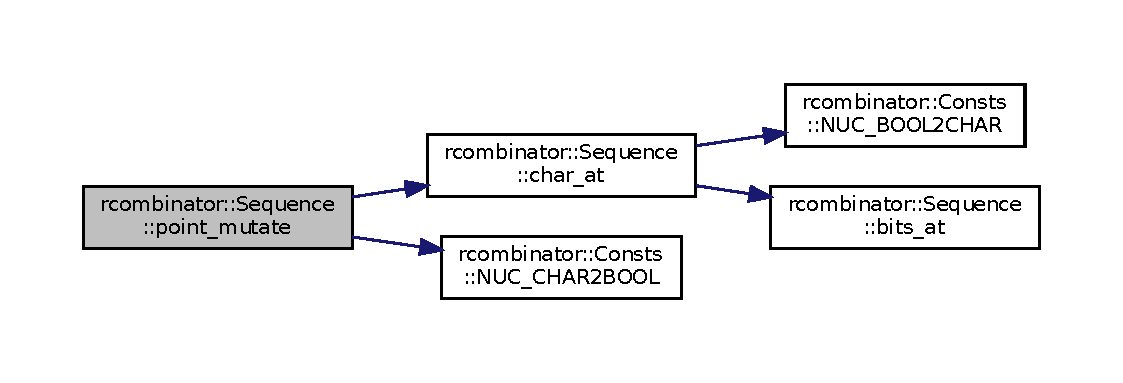
\includegraphics[width=350pt]{classrcombinator_1_1Sequence_a5f7bccd4725bb8c46f6b93bd01a6b2f0_cgraph}
\end{center}
\end{figure}
Here is the caller graph for this function\+:\nopagebreak
\begin{figure}[H]
\begin{center}
\leavevmode
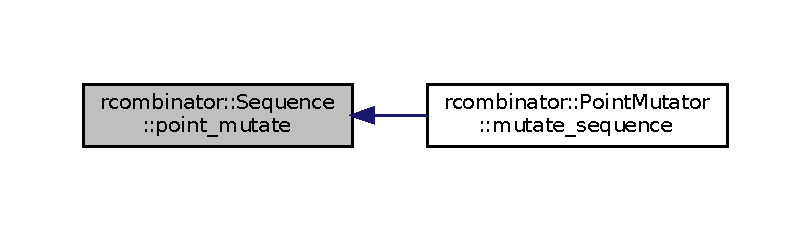
\includegraphics[width=350pt]{classrcombinator_1_1Sequence_a5f7bccd4725bb8c46f6b93bd01a6b2f0_icgraph}
\end{center}
\end{figure}


\subsection{Friends And Related Function Documentation}
\mbox{\Hypertarget{classrcombinator_1_1Sequence_abdc71a8f6617dcb6ab73f0e07eb63b67}\label{classrcombinator_1_1Sequence_abdc71a8f6617dcb6ab73f0e07eb63b67}} 
\index{rcombinator\+::\+Sequence@{rcombinator\+::\+Sequence}!operator$\ast$@{operator$\ast$}}
\index{operator$\ast$@{operator$\ast$}!rcombinator\+::\+Sequence@{rcombinator\+::\+Sequence}}
\subsubsection{\texorpdfstring{operator$\ast$}{operator*}}
{\footnotesize\ttfamily long operator$\ast$ (\begin{DoxyParamCaption}\item[{const \mbox{\hyperlink{classrcombinator_1_1Sequence}{Sequence}} \&}]{s1,  }\item[{const \mbox{\hyperlink{classrcombinator_1_1Sequence}{Sequence}} \&}]{s2 }\end{DoxyParamCaption})\hspace{0.3cm}{\ttfamily [friend]}}



Computes pairwise distances between two sequences. 

This is the standard edit distance score, and is the number of mismatches (because insertions and deletions are not possible in this system). 

\subsection{Member Data Documentation}
\mbox{\Hypertarget{classrcombinator_1_1Sequence_ab37aa0bdc97b3d923407e3a7e17b3209}\label{classrcombinator_1_1Sequence_ab37aa0bdc97b3d923407e3a7e17b3209}} 
\index{rcombinator\+::\+Sequence@{rcombinator\+::\+Sequence}!bases@{bases}}
\index{bases@{bases}!rcombinator\+::\+Sequence@{rcombinator\+::\+Sequence}}
\subsubsection{\texorpdfstring{bases}{bases}}
{\footnotesize\ttfamily std\+::vector$<$bool$>$ rcombinator\+::\+Sequence\+::bases\hspace{0.3cm}{\ttfamily [private]}}



Actual sequence of nucleotides. 

Stored as a string internally. \mbox{\Hypertarget{classrcombinator_1_1Sequence_abb45023862671bbc450bdea543e72165}\label{classrcombinator_1_1Sequence_abb45023862671bbc450bdea543e72165}} 
\index{rcombinator\+::\+Sequence@{rcombinator\+::\+Sequence}!global\+\_\+sequence\+\_\+count@{global\+\_\+sequence\+\_\+count}}
\index{global\+\_\+sequence\+\_\+count@{global\+\_\+sequence\+\_\+count}!rcombinator\+::\+Sequence@{rcombinator\+::\+Sequence}}
\subsubsection{\texorpdfstring{global\+\_\+sequence\+\_\+count}{global\_sequence\_count}}
{\footnotesize\ttfamily long rcombinator\+::\+Sequence\+::global\+\_\+sequence\+\_\+count = 0\hspace{0.3cm}{\ttfamily [static]}, {\ttfamily [private]}}



An internal counter that is incremented every time a sequence is created. 

Used to assign each sequence a unique tag. \mbox{\Hypertarget{classrcombinator_1_1Sequence_abbef2567c1f68239c80769db85455b00}\label{classrcombinator_1_1Sequence_abbef2567c1f68239c80769db85455b00}} 
\index{rcombinator\+::\+Sequence@{rcombinator\+::\+Sequence}!lethal\+\_\+mutations@{lethal\+\_\+mutations}}
\index{lethal\+\_\+mutations@{lethal\+\_\+mutations}!rcombinator\+::\+Sequence@{rcombinator\+::\+Sequence}}
\subsubsection{\texorpdfstring{lethal\+\_\+mutations}{lethal\_mutations}}
{\footnotesize\ttfamily lethal\+\_\+mutations\+\_\+type rcombinator\+::\+Sequence\+::lethal\+\_\+mutations\hspace{0.3cm}{\ttfamily [private]}}



Positions of mutations that are lethal. 

Internally stored as a set. This set is always a subset of {\ttfamily mutations.\+keys}. \mbox{\Hypertarget{classrcombinator_1_1Sequence_a8aac49ef635b95fe0088e5fb59e2bce7}\label{classrcombinator_1_1Sequence_a8aac49ef635b95fe0088e5fb59e2bce7}} 
\index{rcombinator\+::\+Sequence@{rcombinator\+::\+Sequence}!mutations@{mutations}}
\index{mutations@{mutations}!rcombinator\+::\+Sequence@{rcombinator\+::\+Sequence}}
\subsubsection{\texorpdfstring{mutations}{mutations}}
{\footnotesize\ttfamily \mbox{\hyperlink{classrcombinator_1_1Sequence_a95c6d1eea79f9551118a4c988433e5b7}{mutations\+\_\+type}} rcombinator\+::\+Sequence\+::mutations\hspace{0.3cm}{\ttfamily [private]}}



Positions of mutations and what the {\itshape original} nucleotide was. 

Stored as an unordered map locally. \mbox{\Hypertarget{classrcombinator_1_1Sequence_a9f9a2f4654d8b0e0cdb3061b9e0775d7}\label{classrcombinator_1_1Sequence_a9f9a2f4654d8b0e0cdb3061b9e0775d7}} 
\index{rcombinator\+::\+Sequence@{rcombinator\+::\+Sequence}!tag@{tag}}
\index{tag@{tag}!rcombinator\+::\+Sequence@{rcombinator\+::\+Sequence}}
\subsubsection{\texorpdfstring{tag}{tag}}
{\footnotesize\ttfamily long rcombinator\+::\+Sequence\+::tag\hspace{0.3cm}{\ttfamily [private]}}



A number that uniquely identifies this sequence. 

This tag transcends activity (if an inactive sequence becomes active again, it has the same tag) 

The documentation for this class was generated from the following files\+:\begin{DoxyCompactItemize}
\item 
src/\mbox{\hyperlink{sequence_8h}{sequence.\+h}}\item 
src/sequence.\+cpp\end{DoxyCompactItemize}

\hypertarget{structrcombinator_1_1Utils_1_1SummaryStats}{}\section{rcombinator\+:\+:Utils\+:\+:Summary\+Stats$<$ T, T\+\_\+cont $>$ Struct Template Reference}
\label{structrcombinator_1_1Utils_1_1SummaryStats}\index{rcombinator\+::\+Utils\+::\+Summary\+Stats$<$ T, T\+\_\+cont $>$@{rcombinator\+::\+Utils\+::\+Summary\+Stats$<$ T, T\+\_\+cont $>$}}


Plain-\/\+Old-\/\+Data struct to store summary statistics for a list of values.  




{\ttfamily \#include $<$utilities.\+h$>$}

\subsection*{Public Attributes}
\begin{DoxyCompactItemize}
\item 
\mbox{\Hypertarget{structrcombinator_1_1Utils_1_1SummaryStats_a298556c55f80ec5341f68e4437175290}\label{structrcombinator_1_1Utils_1_1SummaryStats_a298556c55f80ec5341f68e4437175290}} 
T \mbox{\hyperlink{structrcombinator_1_1Utils_1_1SummaryStats_a298556c55f80ec5341f68e4437175290}{min}}
\begin{DoxyCompactList}\small\item\em Minimum. \end{DoxyCompactList}\item 
\mbox{\Hypertarget{structrcombinator_1_1Utils_1_1SummaryStats_aee0b73cf97c3992b2924007ab7cf7677}\label{structrcombinator_1_1Utils_1_1SummaryStats_aee0b73cf97c3992b2924007ab7cf7677}} 
T\+\_\+cont \mbox{\hyperlink{structrcombinator_1_1Utils_1_1SummaryStats_aee0b73cf97c3992b2924007ab7cf7677}{q25}}
\begin{DoxyCompactList}\small\item\em First quartile, 25th percentile. \end{DoxyCompactList}\item 
\mbox{\Hypertarget{structrcombinator_1_1Utils_1_1SummaryStats_aaef96ba301012a1d3620dc8a57c68af7}\label{structrcombinator_1_1Utils_1_1SummaryStats_aaef96ba301012a1d3620dc8a57c68af7}} 
T\+\_\+cont \mbox{\hyperlink{structrcombinator_1_1Utils_1_1SummaryStats_aaef96ba301012a1d3620dc8a57c68af7}{median}}
\begin{DoxyCompactList}\small\item\em Median. \end{DoxyCompactList}\item 
\mbox{\Hypertarget{structrcombinator_1_1Utils_1_1SummaryStats_a8d8b1e856b0cee4474297ce3fc5bc702}\label{structrcombinator_1_1Utils_1_1SummaryStats_a8d8b1e856b0cee4474297ce3fc5bc702}} 
T\+\_\+cont \mbox{\hyperlink{structrcombinator_1_1Utils_1_1SummaryStats_a8d8b1e856b0cee4474297ce3fc5bc702}{q75}}
\begin{DoxyCompactList}\small\item\em Third quartile, 75th percentile. \end{DoxyCompactList}\item 
\mbox{\Hypertarget{structrcombinator_1_1Utils_1_1SummaryStats_a0b47d0ce5dab397ba9595573a988051c}\label{structrcombinator_1_1Utils_1_1SummaryStats_a0b47d0ce5dab397ba9595573a988051c}} 
T \mbox{\hyperlink{structrcombinator_1_1Utils_1_1SummaryStats_a0b47d0ce5dab397ba9595573a988051c}{max}}
\begin{DoxyCompactList}\small\item\em Maximum. \end{DoxyCompactList}\item 
\mbox{\Hypertarget{structrcombinator_1_1Utils_1_1SummaryStats_a02fb885c4b1c828ff5fee577f5206594}\label{structrcombinator_1_1Utils_1_1SummaryStats_a02fb885c4b1c828ff5fee577f5206594}} 
T\+\_\+cont \mbox{\hyperlink{structrcombinator_1_1Utils_1_1SummaryStats_a02fb885c4b1c828ff5fee577f5206594}{mean}}
\begin{DoxyCompactList}\small\item\em Arithmetic mean. \end{DoxyCompactList}\end{DoxyCompactItemize}


\subsection{Detailed Description}
\subsubsection*{template$<$typename T, typename T\+\_\+cont$>$\newline
struct rcombinator\+::\+Utils\+::\+Summary\+Stats$<$ T, T\+\_\+cont $>$}

Plain-\/\+Old-\/\+Data struct to store summary statistics for a list of values. 

Is templated on T and T\+\_\+cont, where T is a numeric type, and T\+\_\+cont is a numeric type that can store fractional parts. Stores the quartiles and the mean for a list of values. 

The documentation for this struct was generated from the following file\+:\begin{DoxyCompactItemize}
\item 
src/\mbox{\hyperlink{utilities_8h}{utilities.\+h}}\end{DoxyCompactItemize}

\hypertarget{classrcombinator_1_1T93Model}{}\section{rcombinator\+:\+:T93\+Model Class Reference}
\label{classrcombinator_1_1T93Model}\index{rcombinator\+::\+T93\+Model@{rcombinator\+::\+T93\+Model}}


Tamura ane Nei 1983 Model.  




{\ttfamily \#include $<$point\+\_\+mutation\+\_\+models.\+h$>$}



Inheritance diagram for rcombinator\+:\+:T93\+Model\+:\nopagebreak
\begin{figure}[H]
\begin{center}
\leavevmode
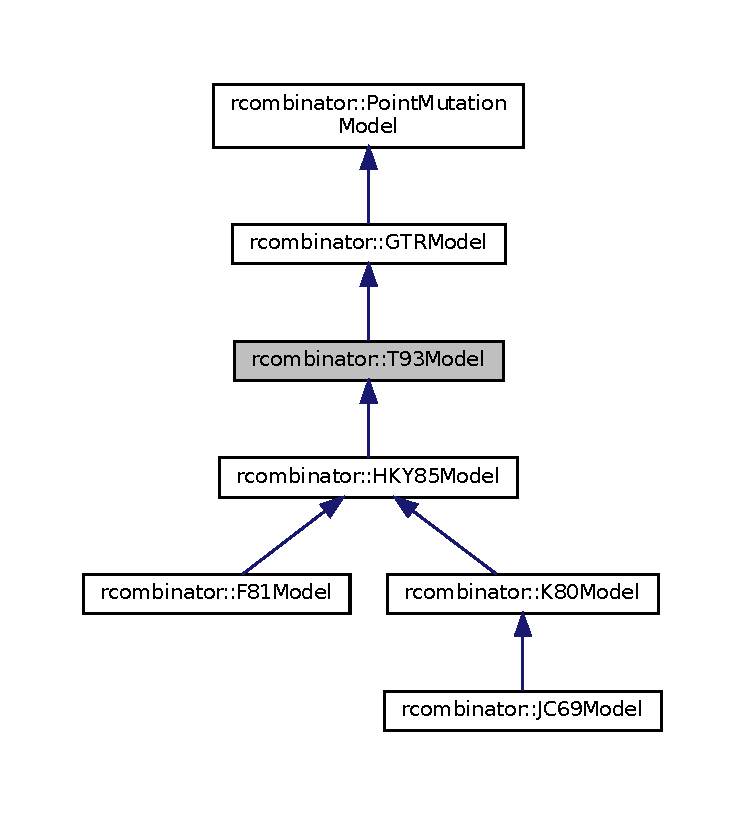
\includegraphics[width=350pt]{classrcombinator_1_1T93Model__inherit__graph}
\end{center}
\end{figure}


Collaboration diagram for rcombinator\+:\+:T93\+Model\+:\nopagebreak
\begin{figure}[H]
\begin{center}
\leavevmode
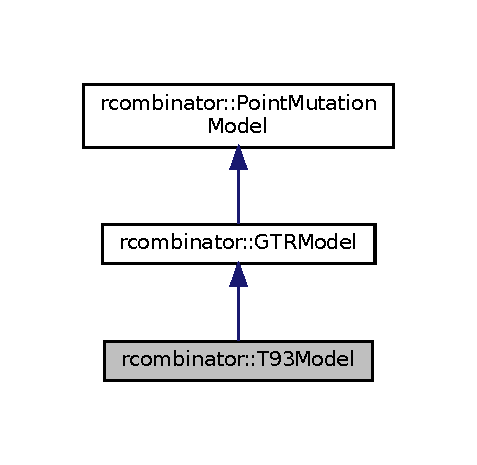
\includegraphics[width=229pt]{classrcombinator_1_1T93Model__coll__graph}
\end{center}
\end{figure}
\subsection*{Public Member Functions}
\begin{DoxyCompactItemize}
\item 
\mbox{\hyperlink{classrcombinator_1_1T93Model_ad857daf369e1d16fc8233b08dc0deef8}{T93\+Model}} (double \mbox{\hyperlink{classrcombinator_1_1GTRModel_a1f58fe556a5ce9aaba6168c9f91e8372}{pi\+\_\+T}}=0.\+25, double pi\+\_\+C=0.\+25, double pi\+\_\+A=0.\+25, double pi\+\_\+G=0.\+25, double \mbox{\hyperlink{classrcombinator_1_1T93Model_a98c3187ba2e9da1f608f17b1e3cf341b}{k1}}=1, double k2=1, double \mbox{\hyperlink{classrcombinator_1_1PointMutationModel_a328a30a438bb1b6a625faa3f714a85c8}{scale}}=1)
\begin{DoxyCompactList}\small\item\em 4 equilibrium base frequency parameters, 2 substitution rate parameters and 1 scale parameter. \end{DoxyCompactList}\end{DoxyCompactItemize}
\subsection*{Protected Member Functions}
\begin{DoxyCompactItemize}
\item 
\mbox{\Hypertarget{classrcombinator_1_1T93Model_aaa8c96927a1ff3b8c611f0d0f9d6f36a}\label{classrcombinator_1_1T93Model_aaa8c96927a1ff3b8c611f0d0f9d6f36a}} 
void \mbox{\hyperlink{classrcombinator_1_1T93Model_aaa8c96927a1ff3b8c611f0d0f9d6f36a}{compute\+\_\+transition\+\_\+matrix}} () override
\begin{DoxyCompactList}\small\item\em Computed by exploiting symmetry. \end{DoxyCompactList}\end{DoxyCompactItemize}
\subsection*{Protected Attributes}
\textbf{ }\par
\begin{DoxyCompactItemize}
\item 
const double \mbox{\hyperlink{classrcombinator_1_1T93Model_a98c3187ba2e9da1f608f17b1e3cf341b}{k1}}
\begin{DoxyCompactList}\small\item\em The subsitution rate parameters. \end{DoxyCompactList}\item 
\mbox{\Hypertarget{classrcombinator_1_1T93Model_a1806ba62860b111c56accc16f1ffdb3d}\label{classrcombinator_1_1T93Model_a1806ba62860b111c56accc16f1ffdb3d}} 
const double {\bfseries k2}
\end{DoxyCompactItemize}

\subsection*{Additional Inherited Members}


\subsection{Detailed Description}
Tamura ane Nei 1983 Model. 

\subsection{Constructor \& Destructor Documentation}
\mbox{\Hypertarget{classrcombinator_1_1T93Model_ad857daf369e1d16fc8233b08dc0deef8}\label{classrcombinator_1_1T93Model_ad857daf369e1d16fc8233b08dc0deef8}} 
\index{rcombinator\+::\+T93\+Model@{rcombinator\+::\+T93\+Model}!T93\+Model@{T93\+Model}}
\index{T93\+Model@{T93\+Model}!rcombinator\+::\+T93\+Model@{rcombinator\+::\+T93\+Model}}
\subsubsection{\texorpdfstring{T93\+Model()}{T93Model()}}
{\footnotesize\ttfamily T93\+Model\+::\+T93\+Model (\begin{DoxyParamCaption}\item[{double}]{pi\+\_\+T = {\ttfamily 0.25},  }\item[{double}]{pi\+\_\+C = {\ttfamily 0.25},  }\item[{double}]{pi\+\_\+A = {\ttfamily 0.25},  }\item[{double}]{pi\+\_\+G = {\ttfamily 0.25},  }\item[{double}]{k1 = {\ttfamily 1},  }\item[{double}]{k2 = {\ttfamily 1},  }\item[{double}]{scale = {\ttfamily 1} }\end{DoxyParamCaption})}



4 equilibrium base frequency parameters, 2 substitution rate parameters and 1 scale parameter. 

pi\+\_\+X = same as for G\+TR k1 = rate of transition T $<$-\/$>$ C when transversion rate is 1 k2 = rate of transition A $<$-\/$>$ G when transversion rate is 1 scale = same as for G\+TR 

\subsection{Member Data Documentation}
\mbox{\Hypertarget{classrcombinator_1_1T93Model_a98c3187ba2e9da1f608f17b1e3cf341b}\label{classrcombinator_1_1T93Model_a98c3187ba2e9da1f608f17b1e3cf341b}} 
\index{rcombinator\+::\+T93\+Model@{rcombinator\+::\+T93\+Model}!k1@{k1}}
\index{k1@{k1}!rcombinator\+::\+T93\+Model@{rcombinator\+::\+T93\+Model}}
\subsubsection{\texorpdfstring{k1}{k1}}
{\footnotesize\ttfamily const double rcombinator\+::\+T93\+Model\+::k1\hspace{0.3cm}{\ttfamily [protected]}}



The subsitution rate parameters. 

Look at the constructor for more details. 

The documentation for this class was generated from the following files\+:\begin{DoxyCompactItemize}
\item 
src/\mbox{\hyperlink{point__mutation__models_8h}{point\+\_\+mutation\+\_\+models.\+h}}\item 
src/point\+\_\+mutation\+\_\+models.\+cpp\end{DoxyCompactItemize}

\chapter{File Documentation}
\hypertarget{constants_8h}{}\doxysection{src/constants.h File Reference}
\label{constants_8h}\index{src/constants.h@{src/constants.h}}


Definitions for enums/constants/functions that are used everywhere.  


{\ttfamily \#include \char`\"{}exception.\+h\char`\"{}}\newline
{\ttfamily \#include $<$cmath$>$}\newline
{\ttfamily \#include $<$set$>$}\newline
{\ttfamily \#include $<$utility$>$}\newline
{\ttfamily \#include $<$vector$>$}\newline
Include dependency graph for constants.\+h\+:
\nopagebreak
\begin{figure}[H]
\begin{center}
\leavevmode
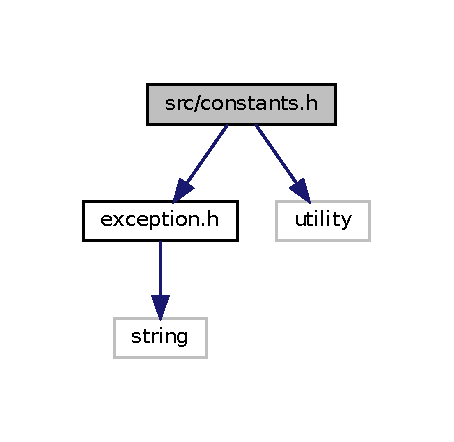
\includegraphics[width=350pt]{constants_8h__incl}
\end{center}
\end{figure}
This graph shows which files directly or indirectly include this file\+:
\nopagebreak
\begin{figure}[H]
\begin{center}
\leavevmode
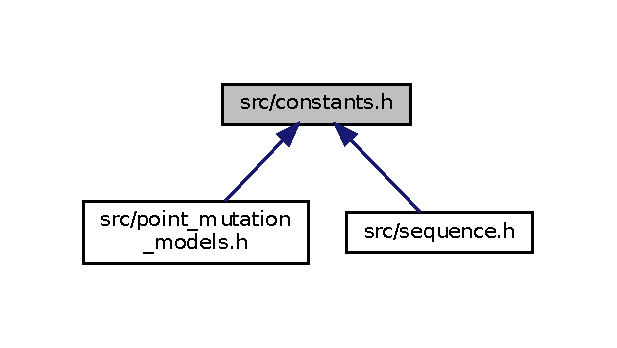
\includegraphics[width=350pt]{constants_8h__dep__incl}
\end{center}
\end{figure}
\doxysubsection*{Namespaces}
\begin{DoxyCompactItemize}
\item 
 \mbox{\hyperlink{namespaceretrocombinator}{retrocombinator}}
\item 
 \mbox{\hyperlink{namespaceretrocombinator_1_1Consts}{retrocombinator\+::\+Consts}}
\end{DoxyCompactItemize}
\doxysubsection*{Typedefs}
\begin{DoxyCompactItemize}
\item 
\mbox{\Hypertarget{namespaceretrocombinator_a47bcd6dd938a6f8e34b0996d940f81ef}\label{namespaceretrocombinator_a47bcd6dd938a6f8e34b0996d940f81ef}} 
typedef double \mbox{\hyperlink{namespaceretrocombinator_a47bcd6dd938a6f8e34b0996d940f81ef}{retrocombinator\+::\+Nuc\+Matrix}}\mbox{[}Consts\+::\+N\+U\+C\+\_\+\+C\+O\+U\+NT\mbox{]}\mbox{[}Consts\+::\+N\+U\+C\+\_\+\+C\+O\+U\+NT\mbox{]}
\begin{DoxyCompactList}\small\item\em Type for transition matrices, rate matrices etc. \end{DoxyCompactList}\item 
\mbox{\Hypertarget{namespaceretrocombinator_a8e1541b50cee66a791df4c437ccbb385}\label{namespaceretrocombinator_a8e1541b50cee66a791df4c437ccbb385}} 
typedef std\+::size\+\_\+t \mbox{\hyperlink{namespaceretrocombinator_a8e1541b50cee66a791df4c437ccbb385}{retrocombinator\+::size\+\_\+type}}
\begin{DoxyCompactList}\small\item\em Type for all indices and sizes. \end{DoxyCompactList}\item 
typedef std\+::set$<$ size\+\_\+type $>$ \mbox{\hyperlink{namespaceretrocombinator_a316667a6633d664fe892bd7e0eb0141e}{retrocombinator\+::cluster\+\_\+type}}
\begin{DoxyCompactList}\small\item\em Types for clustering algorithms. \end{DoxyCompactList}\item 
\mbox{\Hypertarget{namespaceretrocombinator_aa416b6a3a9e444eae3309a16b8607750}\label{namespaceretrocombinator_aa416b6a3a9e444eae3309a16b8607750}} 
typedef std\+::vector$<$ std\+::vector$<$ double $>$ $>$ \mbox{\hyperlink{namespaceretrocombinator_aa416b6a3a9e444eae3309a16b8607750}{retrocombinator\+::dist\+\_\+type}}
\begin{DoxyCompactList}\small\item\em Type for a distance matrix. \end{DoxyCompactList}\item 
\mbox{\Hypertarget{namespaceretrocombinator_a2386ae0e40bc342fbf7ec8b1c16246c1}\label{namespaceretrocombinator_a2386ae0e40bc342fbf7ec8b1c16246c1}} 
typedef std\+::vector$<$ double $>$ \mbox{\hyperlink{namespaceretrocombinator_a2386ae0e40bc342fbf7ec8b1c16246c1}{retrocombinator\+::dist\+\_\+row\+\_\+type}}
\begin{DoxyCompactList}\small\item\em Type for a row in a distance matrix. \end{DoxyCompactList}\item 
\mbox{\Hypertarget{namespaceretrocombinator_afd7c6eb4293e8c4d12827609a9a34b9b}\label{namespaceretrocombinator_afd7c6eb4293e8c4d12827609a9a34b9b}} 
typedef long \mbox{\hyperlink{namespaceretrocombinator_afd7c6eb4293e8c4d12827609a9a34b9b}{retrocombinator\+::tag\+\_\+type}}
\begin{DoxyCompactList}\small\item\em For all integer-\/based codes. \end{DoxyCompactList}\end{DoxyCompactItemize}
\doxysubsection*{Enumerations}
\begin{DoxyCompactItemize}
\item 
enum \mbox{\hyperlink{namespaceretrocombinator_1_1Consts_a274e9195aeee16a2bc05c6c2d13da17d}{retrocombinator\+::\+Consts\+::\+N\+U\+C\+\_\+\+V\+A\+LS}} \{ \newline
\mbox{\hyperlink{namespaceretrocombinator_1_1Consts_a274e9195aeee16a2bc05c6c2d13da17dac9faac145c86659926a2309d19c35dff}{retrocombinator\+::\+Consts\+::T}} = 0, 
\mbox{\hyperlink{namespaceretrocombinator_1_1Consts_a274e9195aeee16a2bc05c6c2d13da17da8a12357162a7bf22e8578359a62411c6}{retrocombinator\+::\+Consts\+::C}} = 1, 
\mbox{\hyperlink{namespaceretrocombinator_1_1Consts_a274e9195aeee16a2bc05c6c2d13da17da6c53f477e84902529dcca14ae060567e}{retrocombinator\+::\+Consts\+::A}} = 2, 
\mbox{\hyperlink{namespaceretrocombinator_1_1Consts_a274e9195aeee16a2bc05c6c2d13da17da06ef41de5b2c3014ce080d3ecece5c4e}{retrocombinator\+::\+Consts\+::G}} = 3, 
\newline
\mbox{\hyperlink{namespaceretrocombinator_1_1Consts_a274e9195aeee16a2bc05c6c2d13da17da4267c64ef80aa3023d8e808832e04b4e}{retrocombinator\+::\+Consts\+::\+N\+U\+C\+\_\+\+C\+O\+U\+NT}} = 4
 \}
\begin{DoxyCompactList}\small\item\em This defines an ordering on the nucleotides, it is used for arrays and transition matrices that work on nucleotides. \end{DoxyCompactList}\end{DoxyCompactItemize}
\doxysubsection*{Functions}
\begin{DoxyCompactItemize}
\item 
\mbox{\Hypertarget{namespaceretrocombinator_1_1Consts_a4f7296df50158c4273a1c5300c24c2f7}\label{namespaceretrocombinator_1_1Consts_a4f7296df50158c4273a1c5300c24c2f7}} 
char \mbox{\hyperlink{namespaceretrocombinator_1_1Consts_a4f7296df50158c4273a1c5300c24c2f7}{retrocombinator\+::\+Consts\+::\+N\+U\+C\+\_\+\+I\+N\+T2\+C\+H\+AR}} (int index)
\begin{DoxyCompactList}\small\item\em Returns a character corresponding a nucleotide given its index. \end{DoxyCompactList}\item 
\mbox{\Hypertarget{namespaceretrocombinator_1_1Consts_a074bd1a42191d4770f74beb2bf228111}\label{namespaceretrocombinator_1_1Consts_a074bd1a42191d4770f74beb2bf228111}} 
int \mbox{\hyperlink{namespaceretrocombinator_1_1Consts_a074bd1a42191d4770f74beb2bf228111}{retrocombinator\+::\+Consts\+::\+N\+U\+C\+\_\+\+C\+H\+A\+R2\+I\+NT}} (char nucleotide)
\begin{DoxyCompactList}\small\item\em Returns the index of a nucleotide given its character form. \end{DoxyCompactList}\item 
\mbox{\Hypertarget{namespaceretrocombinator_1_1Consts_a95eb077a2bba2fe988b44e68a3284314}\label{namespaceretrocombinator_1_1Consts_a95eb077a2bba2fe988b44e68a3284314}} 
std\+::pair$<$ bool, bool $>$ \mbox{\hyperlink{namespaceretrocombinator_1_1Consts_a95eb077a2bba2fe988b44e68a3284314}{retrocombinator\+::\+Consts\+::\+N\+U\+C\+\_\+\+C\+H\+A\+R2\+B\+O\+OL}} (char nucleotide)
\begin{DoxyCompactList}\small\item\em Returns the 2bit-\/encoding of a nucleotide given its character form. \end{DoxyCompactList}\item 
\mbox{\Hypertarget{namespaceretrocombinator_1_1Consts_af335f61cbdfff27175d7f41cd95d426d}\label{namespaceretrocombinator_1_1Consts_af335f61cbdfff27175d7f41cd95d426d}} 
char \mbox{\hyperlink{namespaceretrocombinator_1_1Consts_af335f61cbdfff27175d7f41cd95d426d}{retrocombinator\+::\+Consts\+::\+N\+U\+C\+\_\+\+B\+O\+O\+L2\+C\+H\+AR}} (std\+::pair$<$ bool, bool $>$ bits)
\begin{DoxyCompactList}\small\item\em Returns the character of a nucleotide given its 2bit-\/encoding. \end{DoxyCompactList}\item 
\mbox{\Hypertarget{namespaceretrocombinator_a04664f475f33337cf2a7a4a0b0e3125c}\label{namespaceretrocombinator_a04664f475f33337cf2a7a4a0b0e3125c}} 
const typedef double($\ast$ \mbox{\hyperlink{namespaceretrocombinator_a04664f475f33337cf2a7a4a0b0e3125c}{retrocombinator\+::\+Returns\+Nuc\+Matrix}} ())\mbox{[}Consts\+::\+N\+U\+C\+\_\+\+C\+O\+U\+NT\mbox{]}
\begin{DoxyCompactList}\small\item\em Type for functions that return Nuc\+Matrix and accept no parameters. \end{DoxyCompactList}\item 
\mbox{\Hypertarget{namespaceretrocombinator_a4cbfa6c71aed12291a2875e9f4ce1438}\label{namespaceretrocombinator_a4cbfa6c71aed12291a2875e9f4ce1438}} 
const typedef double($\ast$ \mbox{\hyperlink{namespaceretrocombinator_a4cbfa6c71aed12291a2875e9f4ce1438}{retrocombinator\+::\+Returns\+Nuc\+Matrix\+From\+Double}} (double))\mbox{[}Consts\+::\+N\+U\+C\+\_\+\+C\+O\+U\+NT\mbox{]}
\begin{DoxyCompactList}\small\item\em Type for functions that return Nuc\+Matrix and accept time as parameter. \end{DoxyCompactList}\end{DoxyCompactItemize}
\doxysubsection*{Variables}
\begin{DoxyCompactItemize}
\item 
\mbox{\Hypertarget{namespaceretrocombinator_1_1Consts_a2b743049e71f91009273f493c164679a}\label{namespaceretrocombinator_1_1Consts_a2b743049e71f91009273f493c164679a}} 
const double \mbox{\hyperlink{namespaceretrocombinator_1_1Consts_a2b743049e71f91009273f493c164679a}{retrocombinator\+::\+Consts\+::\+D\+O\+U\+B\+L\+E\+\_\+\+T\+O\+L\+E\+R\+A\+N\+CE}} = pow(10.\+0, -\/8)
\begin{DoxyCompactList}\small\item\em Tolerance for operations on variables of datatype double. \end{DoxyCompactList}\item 
const double \mbox{\hyperlink{namespaceretrocombinator_1_1Consts_ac72fd4ec7b9dc3b42523a83cd69eaee2}{retrocombinator\+::\+Consts\+::\+K80\+\_\+K}} = 10
\begin{DoxyCompactList}\small\item\em Defaults for different point mutation models. \end{DoxyCompactList}\item 
\mbox{\Hypertarget{namespaceretrocombinator_1_1Consts_a49787213bbb5ff96754671440c758270}\label{namespaceretrocombinator_1_1Consts_a49787213bbb5ff96754671440c758270}} 
const double \mbox{\hyperlink{namespaceretrocombinator_1_1Consts_a49787213bbb5ff96754671440c758270}{retrocombinator\+::\+Consts\+::\+K80\+\_\+\+S\+C\+A\+LE}} = 0.\+01
\begin{DoxyCompactList}\small\item\em Default scale for a K80 point mutation model. \end{DoxyCompactList}\item 
\mbox{\Hypertarget{namespaceretrocombinator_1_1Consts_aeeeb7201b2611b428004059f329473ba}\label{namespaceretrocombinator_1_1Consts_aeeeb7201b2611b428004059f329473ba}} 
const double \mbox{\hyperlink{namespaceretrocombinator_1_1Consts_aeeeb7201b2611b428004059f329473ba}{retrocombinator\+::\+Consts\+::\+J\+C69\+\_\+\+S\+C\+A\+LE}} = 0.\+1
\begin{DoxyCompactList}\small\item\em Default scale for a J\+C69 point mutation model. \end{DoxyCompactList}\item 
\mbox{\Hypertarget{namespaceretrocombinator_1_1Consts_af4adf5f1b75ede326285e110e2acf837}\label{namespaceretrocombinator_1_1Consts_af4adf5f1b75ede326285e110e2acf837}} 
const tag\+\_\+type \mbox{\hyperlink{namespaceretrocombinator_1_1Consts_af4adf5f1b75ede326285e110e2acf837}{retrocombinator\+::\+Consts\+::\+I\+N\+I\+T\+\_\+\+F\+A\+M\+I\+L\+Y\+\_\+\+C\+O\+U\+NT}} = -\/1
\begin{DoxyCompactList}\small\item\em The family tag to represent initial sequences in a simulation. \end{DoxyCompactList}\end{DoxyCompactItemize}


\doxysubsection{Detailed Description}
Definitions for enums/constants/functions that are used everywhere. 

More specifically,
\begin{DoxyItemize}
\item biological constants (things like nucleotide names, a fixed nucleotide ordering etc),
\item implementation specific typedefs and constants 
\end{DoxyItemize}
\hypertarget{exception_8h}{}\doxysection{src/exception.h File Reference}
\label{exception_8h}\index{src/exception.h@{src/exception.h}}
{\ttfamily \#include $<$string$>$}\newline
Include dependency graph for exception.\+h\+:
\nopagebreak
\begin{figure}[H]
\begin{center}
\leavevmode
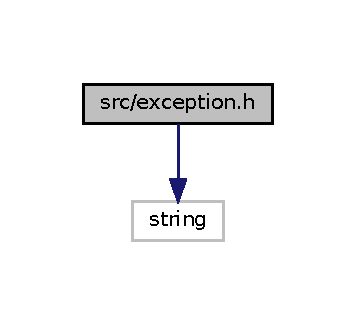
\includegraphics[width=171pt]{exception_8h__incl}
\end{center}
\end{figure}
This graph shows which files directly or indirectly include this file\+:
\nopagebreak
\begin{figure}[H]
\begin{center}
\leavevmode
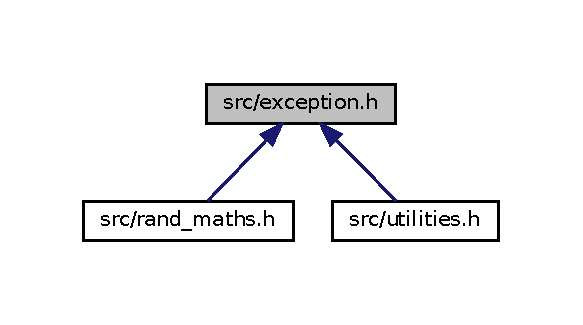
\includegraphics[width=350pt]{exception_8h__dep__incl}
\end{center}
\end{figure}
\doxysubsection*{Classes}
\begin{DoxyCompactItemize}
\item 
class \mbox{\hyperlink{classretrocombinator_1_1Exception}{retrocombinator\+::\+Exception}}
\begin{DoxyCompactList}\small\item\em Basic class to represent exceptions. \end{DoxyCompactList}\end{DoxyCompactItemize}
\doxysubsection*{Namespaces}
\begin{DoxyCompactItemize}
\item 
 \mbox{\hyperlink{namespaceretrocombinator}{retrocombinator}}
\end{DoxyCompactItemize}

\hypertarget{point__mutation__models_8h}{}\doxysection{src/point\+\_\+mutation\+\_\+models.h File Reference}
\label{point__mutation__models_8h}\index{src/point\_mutation\_models.h@{src/point\_mutation\_models.h}}


To store different models of D\+NA evolution.  


{\ttfamily \#include $<$cmath$>$}\newline
{\ttfamily \#include \char`\"{}constants.\+h\char`\"{}}\newline
Include dependency graph for point\+\_\+mutation\+\_\+models.\+h\+:
\nopagebreak
\begin{figure}[H]
\begin{center}
\leavevmode
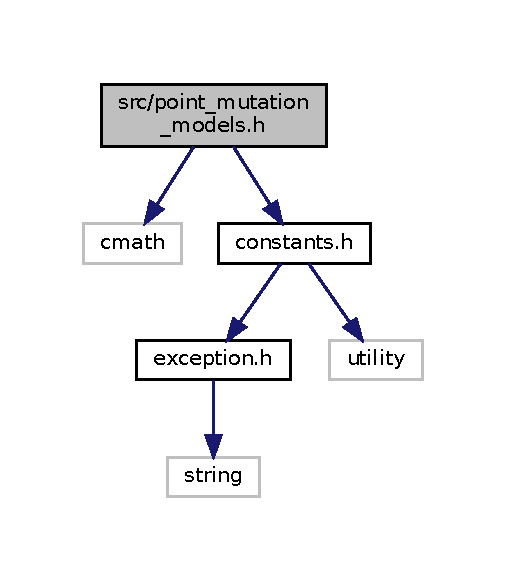
\includegraphics[width=350pt]{point__mutation__models_8h__incl}
\end{center}
\end{figure}
This graph shows which files directly or indirectly include this file\+:
\nopagebreak
\begin{figure}[H]
\begin{center}
\leavevmode
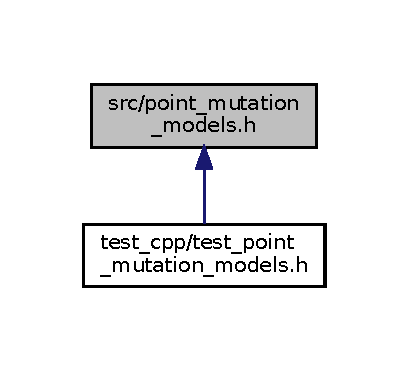
\includegraphics[width=196pt]{point__mutation__models_8h__dep__incl}
\end{center}
\end{figure}
\doxysubsection*{Classes}
\begin{DoxyCompactItemize}
\item 
class \mbox{\hyperlink{classretrocombinator_1_1PointMutationModel}{retrocombinator\+::\+Point\+Mutation\+Model}}
\begin{DoxyCompactList}\small\item\em To represent a model of D\+NA evolution through point mutations. \end{DoxyCompactList}\item 
class \mbox{\hyperlink{classretrocombinator_1_1GTRModel}{retrocombinator\+::\+G\+T\+R\+Model}}
\begin{DoxyCompactList}\small\item\em General Time Reversible Model, Tavare 1986. \end{DoxyCompactList}\item 
class \mbox{\hyperlink{classretrocombinator_1_1TN93Model}{retrocombinator\+::\+T\+N93\+Model}}
\begin{DoxyCompactList}\small\item\em Tamura ane Nei 1983 Model. \end{DoxyCompactList}\item 
class \mbox{\hyperlink{classretrocombinator_1_1HKY85Model}{retrocombinator\+::\+H\+K\+Y85\+Model}}
\begin{DoxyCompactList}\small\item\em Hasegawa, Kishino and Yano 1985 Model. \end{DoxyCompactList}\item 
class \mbox{\hyperlink{classretrocombinator_1_1F81Model}{retrocombinator\+::\+F81\+Model}}
\begin{DoxyCompactList}\small\item\em Felsenstein 1981 Model. \end{DoxyCompactList}\item 
class \mbox{\hyperlink{classretrocombinator_1_1K80Model}{retrocombinator\+::\+K80\+Model}}
\begin{DoxyCompactList}\small\item\em Kimura 2 Parameter Model, 1980. \end{DoxyCompactList}\item 
class \mbox{\hyperlink{classretrocombinator_1_1JC69Model}{retrocombinator\+::\+J\+C69\+Model}}
\begin{DoxyCompactList}\small\item\em Jules and Cantor, 1969. \end{DoxyCompactList}\end{DoxyCompactItemize}
\doxysubsection*{Namespaces}
\begin{DoxyCompactItemize}
\item 
 \mbox{\hyperlink{namespaceretrocombinator}{retrocombinator}}
\end{DoxyCompactItemize}


\doxysubsection{Detailed Description}
To store different models of D\+NA evolution. 

Declares an interface for defintion of different point mutation models. 
\hypertarget{point__mutator_8h}{}\doxysection{src/point\+\_\+mutator.h File Reference}
\label{point__mutator_8h}\index{src/point\_mutator.h@{src/point\_mutator.h}}


To mutate sequences using a point mutation model.  


{\ttfamily \#include $<$string$>$}\newline
{\ttfamily \#include $<$vector$>$}\newline
Include dependency graph for point\+\_\+mutator.\+h\+:
% FIG 0
This graph shows which files directly or indirectly include this file\+:
% FIG 1
\doxysubsection*{Classes}
\begin{DoxyCompactItemize}
\item 
class \mbox{\hyperlink{classretrocombinator_1_1PointMutator}{retrocombinator\+::\+Point\+Mutator}}
\begin{DoxyCompactList}\small\item\em A class that can mutate a given sequence according to a specified point mutation model. \end{DoxyCompactList}\end{DoxyCompactItemize}
\doxysubsection*{Namespaces}
\begin{DoxyCompactItemize}
\item 
 \mbox{\hyperlink{namespaceretrocombinator}{retrocombinator}}
\end{DoxyCompactItemize}


\doxysubsection{Detailed Description}
To mutate sequences using a point mutation model. 

Includes a class which has methods for modifying sequences in place according to some point mutation model. 
\hypertarget{rand__maths_8h}{}\section{src/rand\+\_\+maths.h File Reference}
\label{rand__maths_8h}\index{src/rand\+\_\+maths.\+h@{src/rand\+\_\+maths.\+h}}


Declaration of the global random number generator.  


{\ttfamily \#include \char`\"{}constants.\+h\char`\"{}}\newline
{\ttfamily \#include $<$chrono$>$}\newline
{\ttfamily \#include $<$random$>$}\newline
{\ttfamily \#include $<$set$>$}\newline
Include dependency graph for rand\+\_\+maths.\+h\+:\nopagebreak
\begin{figure}[H]
\begin{center}
\leavevmode
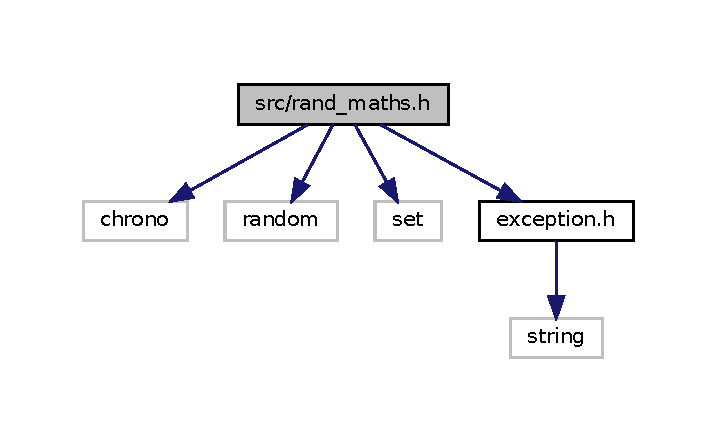
\includegraphics[width=344pt]{rand__maths_8h__incl}
\end{center}
\end{figure}
This graph shows which files directly or indirectly include this file\+:\nopagebreak
\begin{figure}[H]
\begin{center}
\leavevmode
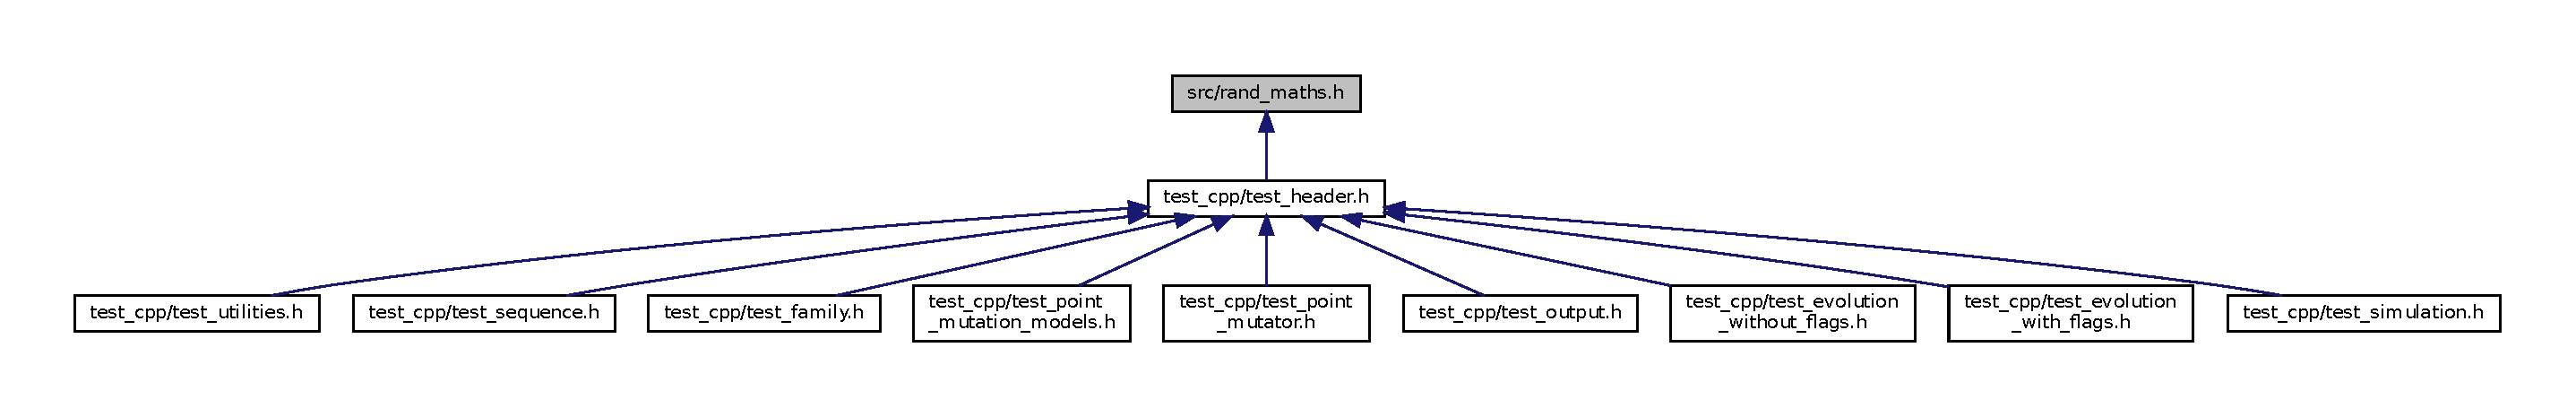
\includegraphics[width=350pt]{rand__maths_8h__dep__incl}
\end{center}
\end{figure}
\subsection*{Classes}
\begin{DoxyCompactItemize}
\item 
class \hyperlink{classretrocombinator_1_1RandMaths}{retrocombinator\+::\+Rand\+Maths}
\begin{DoxyCompactList}\small\item\em For all maths helper functions that use random number generation. \end{DoxyCompactList}\end{DoxyCompactItemize}


\subsection{Detailed Description}
Declaration of the global random number generator. 

Used for basic methods in statistics and probability. R\+NG is the global instance name. 
\hypertarget{sequence_8h}{}\section{src/sequence.h File Reference}
\label{sequence_8h}\index{src/sequence.\+h@{src/sequence.\+h}}


To store a D\+NA sequence and the mutations that it has undergone.  


{\ttfamily \#include \char`\"{}constants.\+h\char`\"{}}\newline
{\ttfamily \#include $<$string$>$}\newline
{\ttfamily \#include $<$unordered\+\_\+map$>$}\newline
{\ttfamily \#include $<$unordered\+\_\+set$>$}\newline
{\ttfamily \#include $<$utility$>$}\newline
{\ttfamily \#include $<$vector$>$}\newline
Include dependency graph for sequence.\+h\+:\nopagebreak
\begin{figure}[H]
\begin{center}
\leavevmode
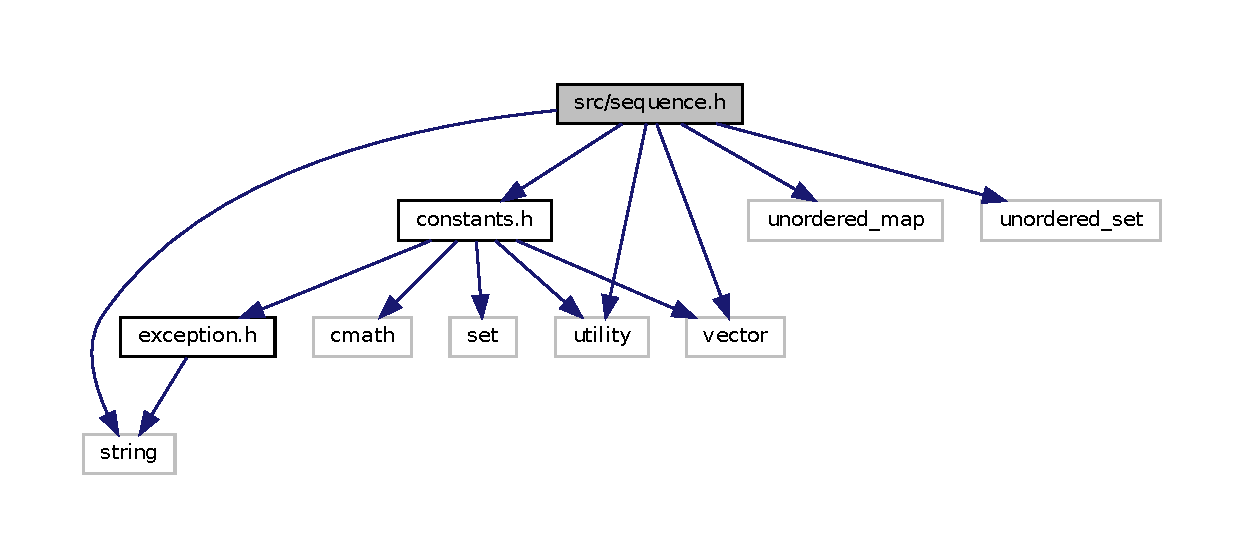
\includegraphics[width=350pt]{sequence_8h__incl}
\end{center}
\end{figure}
This graph shows which files directly or indirectly include this file\+:
\nopagebreak
\begin{figure}[H]
\begin{center}
\leavevmode
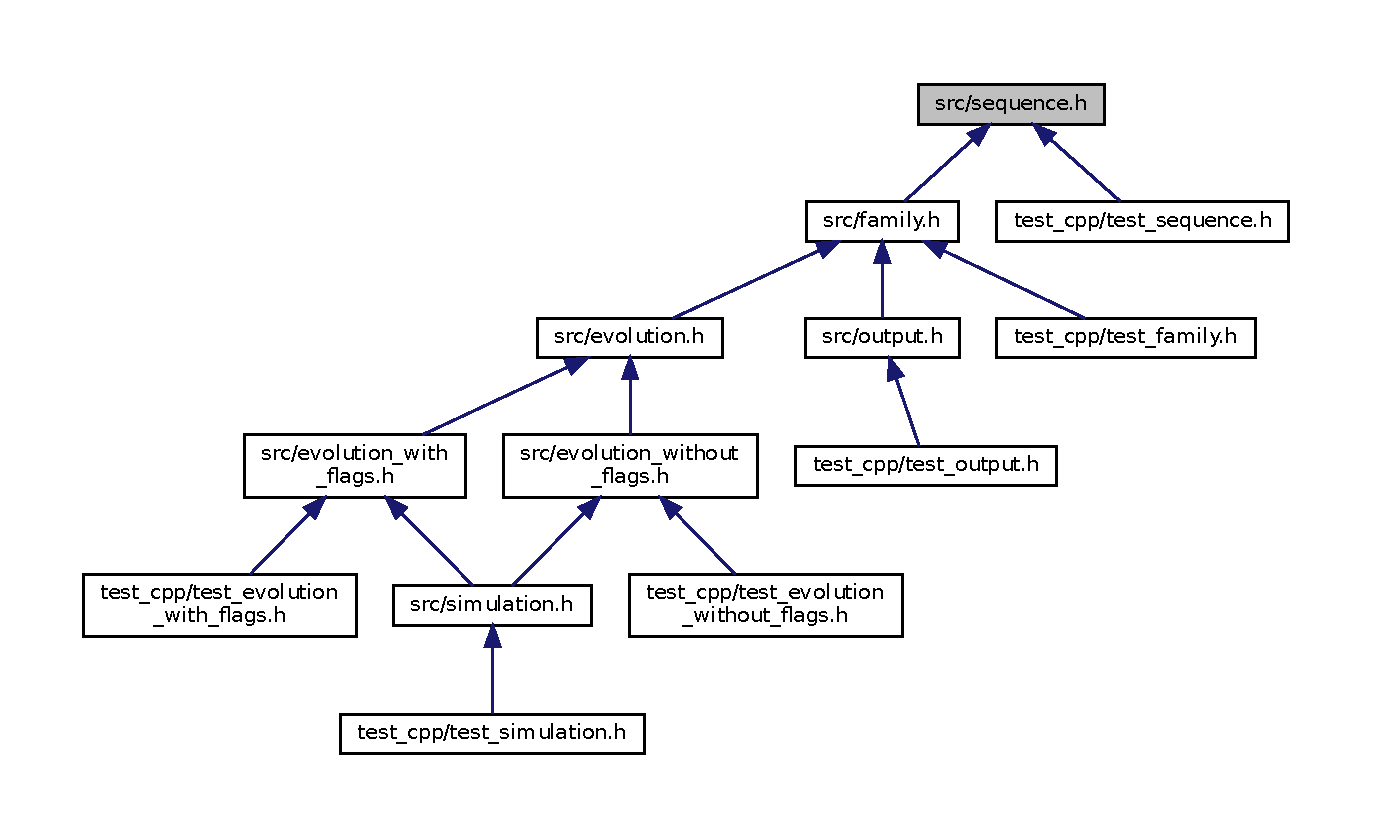
\includegraphics[width=350pt]{sequence_8h__dep__incl}
\end{center}
\end{figure}
\subsection*{Classes}
\begin{DoxyCompactItemize}
\item 
class \mbox{\hyperlink{classrcombinator_1_1Sequence}{rcombinator\+::\+Sequence}}
\begin{DoxyCompactList}\small\item\em To represent a D\+NA sequence and the mutations that it has undergone. \end{DoxyCompactList}\end{DoxyCompactItemize}


\subsection{Detailed Description}
To store a D\+NA sequence and the mutations that it has undergone. 

Includes methods to keep track of which mutations are lethal, methods to recombine sequences and methods to get the pairwise distances between two strings. 
\hypertarget{utilities_8h}{}\section{src/utilities.h File Reference}
\label{utilities_8h}\index{src/utilities.\+h@{src/utilities.\+h}}


Definitions of basic helper functions.  


{\ttfamily \#include $<$algorithm$>$}\newline
{\ttfamily \#include $<$cmath$>$}\newline
{\ttfamily \#include $<$vector$>$}\newline
{\ttfamily \#include \char`\"{}exception.\+h\char`\"{}}\newline
Include dependency graph for utilities.\+h\+:\nopagebreak
\begin{figure}[H]
\begin{center}
\leavevmode
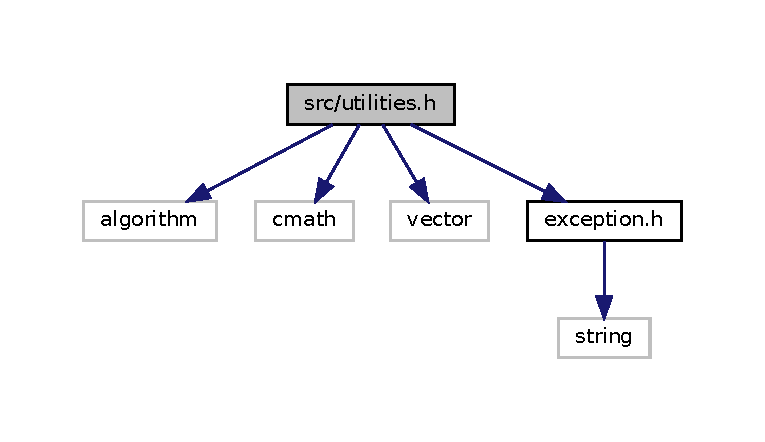
\includegraphics[width=350pt]{utilities_8h__incl}
\end{center}
\end{figure}
\subsection*{Classes}
\begin{DoxyCompactItemize}
\item 
struct \mbox{\hyperlink{structrcombinator_1_1Utils_1_1SummaryStats}{rcombinator\+::\+Utils\+::\+Summary\+Stats$<$ T, T\+\_\+cont $>$}}
\begin{DoxyCompactList}\small\item\em Plain-\/\+Old-\/\+Data struct to store summary statistics for a list of values. \end{DoxyCompactList}\end{DoxyCompactItemize}
\subsection*{Namespaces}
\begin{DoxyCompactItemize}
\item 
 \mbox{\hyperlink{namespacercombinator_1_1Utils}{rcombinator\+::\+Utils}}
\begin{DoxyCompactList}\small\item\em To store some useful functions in a namespace and prevent conflicts. \end{DoxyCompactList}\end{DoxyCompactItemize}
\subsection*{Functions}
\begin{DoxyCompactItemize}
\item 
bool \mbox{\hyperlink{namespacercombinator_1_1Utils_aa38fa31292dbf3a06522dc76b20e2572}{rcombinator\+::\+Utils\+::is\+\_\+in\+\_\+range}} (long test, long lb, long ub)
\begin{DoxyCompactList}\small\item\em Checks whether a number lies within a range. \end{DoxyCompactList}\end{DoxyCompactItemize}


\subsection{Detailed Description}
Definitions of basic helper functions. 

A collection of short, useful functions and data structures 
%--- End generated contents ---

% Index
\backmatter
\newpage
\phantomsection
\clearemptydoublepage
\addcontentsline{toc}{chapter}{Index}
\printindex

\end{document}
